\documentclass[9pt,a4paper]{book}
\usepackage{shevonNotebook}
%标题配置—————————————
\title{线性代数与解析几何\\ \large{ 重要知识点总结}\\ \small{The Summary of Linear Algebra and the Analytic Geometry}\\
	\ \\
	\begin{center}
		\includegraphics[width=10cm]{cover6.png}

	\end{center}
}
\author{关舒文\\\small{\kaishu{华南理工大学}}}
\date{\small{Latest Update\ :\ \today}}
%正文部分—————————————
\begin{document}
%目录与公式编号生成——————————
\numberwithin{equation}{section}
\allowdisplaybreaks%强制自动换行
\newgeometry{left=2cm,right=2cm,marginparwidth=0cm,marginparsep=0cm}%封面设置
\pagenumbering{roman}
\maketitle
\thispagestyle{empty}
%页面重新配置----------------------------
\restoregeometry
{\printnomenclature
\setcounter{page}{0}\pagenumbering{roman}
\addcontentsline{toc}{chapter}{符号说明}}
\newpage
\pagenumbering{Roman}
\setcounter{page}{0}
\tableofcontents



%正文开始—————————————可以使用\boldmath输入粗斜体与\unboldmath合用
\chapter{行列式\\Determinant}
\pagenumbering{arabic}
\setcounter{page}{2}
\section{二阶与三阶行列式}
\begin{defination}[二阶行列式的定义]
	令\[ D= \begin{vmatrix}
	a_{11}&a_{12}\\a_{21}&a_{22}
	\end{vmatrix}=a_{11}a_{22}-a_{12}a_{21} \]其中$ \begin{vmatrix}
		a_{11}&a_{12}\\a_{21}&a_{22}
	\end{vmatrix} $称为\textbf{二阶行列式}\index{EJHLS@二阶行列式},这里$ a_{11},a_{22} $所在的斜线称为二阶行列式的主对角线,相应的$ a_{11},a_{22} $称为\textbf{主对角线元素},而$ a_{12},a_{21} $称为\textbf{副对角线元素}.\index{ZDJXYS@主对角线元素}\index{FDJXYS@副对角线元素}
\end{defination}
\begin{defination}[三阶行列式的定义]
	令\[D={\begin{vmatrix}
		{{a_{11}}}&{{a_{12}}}&{{a_{13}}} \\ 
		{{a_{21}}}&{{a_{22}}}&{{a_{23}}} \\ 
		{{a_{31}}}&{{a_{32}}}&{{a_{33}}} 
		\end{vmatrix}} = {a_{11}}{a_{22}}{a_{33}} + {a_{12}}{a_{23}}{a_{31}} + {a_{13}}{a_{21}}{a_{32}} - {a_{11}}{a_{23}}{a_{32}} - {a_{12}}{a_{21}}{a_{33}} - {a_{13}}{a_{22}}{a_{31}},\]我们称之为\textbf{三阶行列式}.\index{SJHLS@三阶行列式}
\end{defination}
\section{$ n $阶排列及其逆序数,对换}
\begin{defination}[排列的定义]
	由自然数$ 1,2,\cdots,n $组成(不能重复)的任意一个$ n $元有序数组$ i_1i_2\cdots i_n $称为一个\textbf{$ n $阶排列},其中排列$ 12\cdots n  $称为\textbf{自然排列}.\index{PL@排列}\index{ZRPL@自然排列}
\end{defination}
\begin{theorem}
	$ n $阶排列一共有$ n!=(n-1)(n-2)\cdots 3\cdot 2\cdot 1  $个.
\end{theorem}
\begin{defination}
	在一个排列中,如果一个较大的数字排在了一个较小的数字之前,则称这两个数字构成一个\textbf{逆序}.否则,称这两个数字构成一个\textbf{顺序}.两个数字之间的关系只能是顺序或逆序.有以下定义
	\begin{enumerate}
		\item 在一个排列$ i_1i_2\cdots i_n $中,逆序的总数称为这个排列的\textbf{逆序数},记为$ \tau(i_1i_2\cdots i_n) $.
		\item 逆序数为奇数的排列称为\textbf{奇排列},逆序数为偶数的排列称为\textbf{偶排列}.
		\index{LX@逆序}\index{SX@顺序}\index{LXS@逆序数}\index{JPL@奇排列}\index{OPL@偶排列}
	\end{enumerate}
特别地,根据定义我们可得:\begin{enumerate}
	\item 逆序数最小的排列为自然排列,$ \tau(12\cdots n)=0 $;
	\item 逆序数最大的排列为反向自然排列,$ \displaystyle \tau\Bigl( n(n-1)\cdots321\Bigr) =\sum_{i=1}^{n-1}i=\frac{n(n-1)}{2} $.
\end{enumerate}
\end{defination}
\begin{defination}[对换的定义]
	把一个排列中的两个数字$ i,j $的位置互换而保持其余数字的位置不动,则称对这个排列施行了一次\textbf{对换}\index{DH@对换},记作$ (i,j) $.两个相邻位置数字的对换称为\textbf{不相邻对换},否则称为\textbf{一般对换}.\index{BXLDH@不相邻对换}\index{YBDH@一般对换}
\end{defination}
\begin{theorem}
	对换具有可逆性.
\end{theorem}
\begin{theorem}
	对换改变排列的奇偶性.
\end{theorem}
\begin{inference}
	排列经过奇数次对换其奇偶性发生变化,经过偶数次对换其奇偶性不变.
\end{inference}
\begin{inference}
	当$ n\geqslant 2 $时,在$ n $阶排列中,奇偶排列数目相等各有$ \dfrac{n!}{2} $个.
\end{inference}
\begin{theorem}
	自然排列$ 12\cdots n $可以与任意$ n $阶排列$ i_1i_2\cdots i_n $经过一系列对换相互转换,且所作对换次数与排列$ i_1i_2\cdots i_n $具有相同的奇偶性.
\end{theorem}
\section{$ n $阶行列式的定义}
\begin{defination}[$ n $阶行列式的定义]
\[ 	D = {\begin{vmatrix}
		{{a_{11}}}&{{a_{12}}}& \cdots &{{a_{1n}}}\\
		{{a_{21}}}&{{a_{22}}}& \cdots &{{a_{2n}}}\\
		\vdots & \vdots &\;& \vdots \\
		{{a_{n1}}}&{{a_{n2}}}& \cdots &{{a_{nn}}}
		\end{vmatrix}} \]表示一个\textbf{$ n $阶行列式}.其中元素$ a_{ij}\in \mathbb{C}\quad(i,j=1,2,\cdots,n) $.\index{NJHLS@$ n $阶行列式}
\end{defination}
\begin{defination}
	$ n $阶行列式等于所有来自不同行不同列的$ n $个元素乘积的代数和.由于代数和的项数为$ n! $个,为了表达方便,我们可以将每项中的$ n $个元素按行指标有小及大的顺序排列,即写作$ a_{1j_1}a_{2j_2}\cdots a_{nj_n} $的形式,并规定当列指标$ j_1j_2\cdots j_n $是偶排列时,此项前面带正号,若是奇排列则前面带负号.这样,$ n $阶行列式被定义为\[ 	D = {\begin{vmatrix}
		{{a_{11}}}&{{a_{12}}}& \cdots &{{a_{1n}}}\\
		{{a_{21}}}&{{a_{22}}}& \cdots &{{a_{2n}}}\\
		\vdots & \vdots &\;& \vdots \\
		{{a_{n1}}}&{{a_{n2}}}& \cdots &{{a_{nn}}}
		\end{vmatrix}}=\sum_{j_1j_2\cdots j_n}{{(-1)}^{\tau (j_1j_2\cdots j_n)} a_{1j_1}a_{2j_2}\cdots a_{nj_n}}. \]其中$ \displaystyle \sum_{j_1j_2\cdots j_n} $表示对所有可能的$ n $阶排列求和.上式称为\textbf{行列式的展开式}.\index{HLSDZJKS@行列式的展开式}
	
	上述$ n $阶行列式通常记为$ D=\mathrm{det}(a_{ij}) $或着$ |a_{ij}| $.当$ n=1 $时我们规定$ |a_{11}|=a_{11} $.
	
	若行或列指标均不为自然排列,则我们有以下展开式:\[ 	D = {\begin{vmatrix}
		{{a_{11}}}&{{a_{12}}}& \cdots &{{a_{1n}}}\\
		{{a_{21}}}&{{a_{22}}}& \cdots &{{a_{2n}}}\\
		\vdots & \vdots &\;& \vdots \\
		{{a_{n1}}}&{{a_{n2}}}& \cdots &{{a_{nn}}}
		\end{vmatrix}}=\sum_{j_1j_2\cdots j_n}{{(-1)}^{\tau(i_1i_2\cdots i_n)+\tau (j_1j_2\cdots j_n)} a_{i_1j_1}a_{i_2j_2}\cdots a_{i_nj_n}}. \]
\end{defination}
\begin{defination}
	在行列式中,由左上角到右下角所形成的斜线称为\textbf{主对角线},由右上角到左上角所形成的斜线称为\textbf{副对角线}.在主对角线下方的元素全为零,称为\textbf{上三角行列式},如果主对角线上方的元素全为零,则称为\textbf{下三角行列式}.上三角行列式和下三角行列式统称为\textbf{三角行列式}.如果除了主对角线之外的元素全为零,则称为\textbf{对角行列式}.
	\index{ZDJX@主对角线}
	\index{FDJX@副对角线}
	\index{SSJHLS@上三角行列式}
	\index{XSJHLS@下三角行列式}
	\index{SJHLS@三角行列式}
	\index{DJHLS@对角行列式}
\end{defination}
\section{$ n $阶行列式的性质及运算}
\begin{feature}
	行与列互换,行列式的值不变,即 \[ {\begin{vmatrix}
		{{a_{11}}}&{{a_{12}}}& \cdots &{{a_{1n}}}\\
		{{a_{21}}}&{{a_{22}}}& \cdots &{{a_{2n}}}\\
		\vdots & \vdots &{\rm{ }}& \vdots \\
		{{a_{n1}}}&{{a_{n2}}}& \cdots &{{a_{nn}}}
		\end{vmatrix}}  =  {\begin{vmatrix}
		{{a_{11}}}&{{a_{21}}}& \cdots &{{a_{n1}}}\\
		{{a_{12}}}&{{a_{22}}}& \cdots &{{a_{n2}}}\\
		\vdots & \vdots &{\rm{ }}& \vdots \\
		{{a_{1n}}}&{{a_{2n}}}& \cdots &{{a_{nn}}}
		\end{vmatrix}} .\]假设\[ D={\begin{vmatrix}
		{{a_{11}}}&{{a_{12}}}& \cdots &{{a_{1n}}}\\
		{{a_{21}}}&{{a_{22}}}& \cdots &{{a_{2n}}}\\
		\vdots & \vdots &{\rm{ }}& \vdots \\
		{{a_{n1}}}&{{a_{n2}}}& \cdots &{{a_{nn}}}
		\end{vmatrix}} \qquad  D^{\mathrm{T}}{\begin{vmatrix}
		{{a_{11}}}&{{a_{21}}}& \cdots &{{a_{n1}}}\\
		{{a_{12}}}&{{a_{22}}}& \cdots &{{a_{n2}}}\\
		\vdots & \vdots &{\rm{ }}& \vdots \\
		{{a_{1n}}}&{{a_{2n}}}& \cdots &{{a_{nn}}}
		\end{vmatrix}} \]那么称$ D^{\mathrm{T}} $为$ D $的\textbf{转置行列式}\index{ZZHLS@转置行列式},由此性质可知行列式中行与列的地位是对称的,具有相同的性质.上述性质可改写成$ D^{\mathrm{T}}=D $.
\end{feature}
\begin{feature}
	在行列式中,如果某一行(列)元素全为零,则该行列式的值为零.
\end{feature}
\begin{feature}
	交换任意两行(列)的位置,行列式的值变号,即\[ {\begin{vmatrix}
		{{a_{11}}}&{{a_{12}}}& \cdots &{{a_{1n}}}\\
		\vdots & \vdots &{\rm{ }}& \vdots \\
		{{a_{i1}}}&{{a_{i2}}}& \cdots &{{a_{in}}}\\
		\vdots & \vdots &{\rm{ }}& \vdots \\
		{{a_{j1}}}&{{a_{j2}}}& \cdots &{{a_{jn}}}\\
		\vdots & \vdots &{\rm{ }}& \vdots \\
		{{a_{n1}}}&{{a_{n2}}}& \cdots &{{a_{nn}}}
		\end{vmatrix}}  +  {\begin{vmatrix}
		{{a_{11}}}&{{a_{12}}}& \cdots &{{a_{1n}}}\\
		\vdots & \vdots &{\rm{ }}& \vdots \\
		{{a_{j1}}}&{{a_{j2}}}& \cdots &{{a_{jn}}}\\
		\vdots & \vdots &{\rm{ }}& \vdots \\
		{{a_{i1}}}&{{a_{i2}}}& \cdots &{{a_{in}}}\\
		\vdots & \vdots &{\rm{ }}& \vdots \\
		{{a_{n1}}}&{{a_{n2}}}& \cdots &{{a_{nn}}}
		\end{vmatrix}} .\]
\end{feature}
\begin{feature}
	如果行列式有两行(列)完全相同,则行列式为零.
\end{feature}
\begin{feature}
	行列式具有线性型,即
	\begin{enumerate}
		\item\[ {\begin{vmatrix}
			{{a_{11}}}&{{a_{12}}}& \cdots &{{a_{1n}}}\\
			\vdots & \vdots &{\rm{ }}& \vdots \\
			{{b_1} + {c_1}}&{{b_2} + {c_2}}& \cdots &{{b_n} + {c_n}}\\
			\vdots & \vdots &{\rm{ }}& \vdots \\
			{{a_{n1}}}&{{a_{n2}}}& \cdots &{{a_{nn}}}
			\end{vmatrix}}{\rm{ = }} {\begin{vmatrix}
			{{a_{11}}}&{{a_{12}}}& \cdots &{{a_{1n}}}\\
			\vdots & \vdots &{\rm{ }}& \vdots \\
			{{b_1}}&{{b_2}}& \cdots &{{b_n}}\\
			\vdots & \vdots &{\rm{ }}& \vdots \\
			{{a_{n1}}}&{{a_{n2}}}& \cdots &{{a_{nn}}}
			\end{vmatrix}}  +  {\begin{vmatrix}
			{{a_{11}}}&{{a_{12}}}& \cdots &{{a_{1n}}}\\
			\vdots & \vdots &{\rm{ }}& \vdots \\
			{{c_1}}&{{c_2}}& \cdots &{{c_n}}\\
			\vdots & \vdots &{\rm{ }}& \vdots \\
			{{a_{n1}}}&{{a_{n2}}}& \cdots &{{a_{nn}}}
			\end{vmatrix}} ;\] 
		\item\[ {\begin{vmatrix}
			{{a_{11}}}&{{a_{12}}}& \cdots &{{a_{1n}}}\\
			\vdots & \vdots &{\rm{ }}& \vdots \\
			{k{a_{i1}}}&{k{a_{i2}}}& \cdots &{k{a_{in}}}\\
			\vdots & \vdots &{\rm{ }}& \vdots \\
			{{a_{n1}}}&{{a_{n2}}}& \cdots &{{a_{nn}}}
			\end{vmatrix}}  = k {\begin{vmatrix}
			{{a_{11}}}&{{a_{12}}}& \cdots &{{a_{1n}}}\\
			\vdots & \vdots &{\rm{ }}& \vdots \\
			{{a_{i1}}}&{{a_{i2}}}& \cdots &{{a_{in}}}\\
			\vdots & \vdots &{\rm{ }}& \vdots \\
			{{a_{n1}}}&{{a_{n2}}}& \cdots &{{a_{nn}}}
			\end{vmatrix}} .\]
	\end{enumerate}
\end{feature}
\begin{feature}
	如果行列式有两行(列)成比例,则行列式为零,即\[  {\begin{vmatrix}
		{{a_{11}}}&{{a_{12}}}& \cdots &{{a_{1n}}}\\
		\vdots & \vdots &{\rm{ }}& \vdots \\
		{{a_{i1}}}&{{a_{i2}}}& \cdots &{{a_{in}}}\\
		\vdots & \vdots &{\rm{ }}& \vdots \\
		{k{a_{i1}}}&{k{a_{i2}}}& \cdots &{k{a_{in}}}\\
		\vdots & \vdots &{\rm{ }}& \vdots \\
		{{a_{n1}}}&{{a_{n2}}}& \cdots &{{a_{nn}}}
		\end{vmatrix}} =0. \]
\end{feature}
\begin{feature}
	行列式某一行(列)的$ k $倍加到令一行(列),行列式的值不变,即\[  {\begin{vmatrix}
		{{a_{11}}}&{{a_{12}}}& \cdots &{{a_{1n}}}\\
		\vdots & \vdots &{\rm{ }}& \vdots \\
		{{a_{i1}}}&{{a_{i2}}}& \cdots &{{a_{in}}}\\
		\vdots & \vdots &{\rm{ }}& \vdots \\
		{{a_{j1}}}&{{a_{j2}}}& \cdots &{{a_{jn}}}\\
		\vdots & \vdots &{\rm{ }}& \vdots \\
		{{a_{n1}}}&{{a_{n2}}}& \cdots &{{a_{nn}}}
		\end{vmatrix}} {\rm{ = }} {\begin{vmatrix}
		{{a_{11}}}&{{a_{12}}}& \cdots &{{a_{1n}}}\\
		\vdots & \vdots &{\rm{ }}& \vdots \\
		{{a_{i1}}}&{{a_{i2}}}& \cdots &{{a_{in}}}\\
		\vdots & \vdots &{\rm{ }}& \vdots \\
		{{a_{j1}} + k{a_{i1}}}&{{a_{j2}}{\rm{ + }}k{a_{i2}}}& \cdots &{{a_{jn}}{\rm{ + }}k{a_{in}}}\\
		\vdots & \vdots &{\rm{ }}& \vdots \\
		{{a_{n1}}}&{{a_{n2}}}& \cdots &{{a_{nn}}}
		\end{vmatrix}} . \]
\end{feature}
\begin{defination}
	我们引入如下记号以描述行列式的变形:
	\begin{enumerate}
		\item $ r_i\div k $(或 $ c_i\div k $)表示从第$ i $行(列)提取公因子$ k $;
		\item $ r_i+kr_j $(或$ c_i+kc_j $)表示将第$ j $行(列)的$ k $倍加到第$ i $行(列);
		\item $ r_i\leftrightarrow r_j $(或$ c_i\leftrightarrow c_j $)表示交换第$ i $行(列)与第$ j $行(列)的位置.
	\end{enumerate}
\end{defination}
\section{行列式按一行展开及克拉默法则}
\section{八大类型行列式及其解法}
\subsection{}

\chapter{矩阵\\Matrix}
\section{矩阵及其运算}
\section{矩阵的分块}
\section{矩阵的秩}
\section{矩阵的逆}
\section{初等矩阵}
\chapter{向量代数与几何应用\\Vector Algebra and Geometry}
\section{向量的线性运算与空间直角坐标系}
\section{向量的内积,外积与混合积}
\section{空间平面及其方程}
\section{空间直线及其方程}
\chapter{线性方程组\\System of Linear Equations}
\section{消元法}
\begin{defination}[相容方程组与不相容方程组的定义]
	\index{XRFCZ@相容方程组}
	\index{BXRFCZ@不相容方程组}
	有解的方程组称为\textbf{相容方程组};没有解的方程组称为\textbf{不相容方程组}.
\end{defination}
\begin{defination}
	设给定两个线性方程组.如果第一个方程组的解都是第二个方程组的解,同时第二个方程组的解也都是第一个方程组的解,则称他们是\textbf{同解方程组}.
	\index{TJFCZ@同解方程组}
	对于下述线性方程组:
	\begin{equation}\label{xxfcz}
		\left\{
		\begin{array}{c}
		a_{11}x_1+a_{12}x_2+\cdots+a_{1n}x_n=b_1\\
		a_{21}x_1+a_{22}x_2+\cdots+a_{2n}x_n=b_2\\
		\vdots \\
		a_{m1}x_1+a_{m2}x_2+\cdots+a_{mn}x_n=b_m
		\end{array}
		\right.,
	\end{equation}
	\index{XSJZ@系数矩阵}
	\index{WZLJZ@未知量矩阵}
	\index{CSXJZ@常数项矩阵}
	若令\[
	\text{系数矩阵}\ \bm{A}=\begin{bmatrix}
			a_{11} & a_{12} & \cdots & a_{1n}\\
			a_{21} & a_{22} & \cdots & a_{2n}\\
			\vdots & \vdots & \      & \vdots\\
			a_{m1} & a_{m2} & \cdots & a_{mn}
							\end{bmatrix},
	\text{未知量矩阵}\ \bm{X}=\begin{bmatrix}
								x_1\\
								x_2\\
								\vdots\\
								x_n
							\end{bmatrix},
	\text{常数项矩阵}\ \bm{b}=\begin{bmatrix}
	b_1\\
	b_2\\
	\vdots\\
	b_n
	\end{bmatrix},
	\]
	则方程组\ref{xxfcz}可以改写成矩阵的形式\[ \bm{AX}=\bm{b}, \]
	称$ \bm{A} $为方程组\ref{xxfcz}的系数矩阵,而
	$$
	\widetilde{\bm{A}}=[\bm{A}|\bm{b}]=
	\left[
	\begin{array}{cccc|c}
	a_{11} & a_{12} & \cdots & a_{1n}&b_1\\
	a_{21} & a_{22} & \cdots & a_{2n}&b_2\\
	\vdots & \vdots & \      & \vdots&\vdots\\
	a_{m1} & a_{m2} & \cdots & a_{mn}&b_m
	\end{array}
	\right]
	 $$
	 称为方程组\ref{xxfcz}的\textbf{增广矩阵}.其中增广矩阵唯一确定线性方程组.
	 \index{ZGJZ@增广矩阵}
	 \nomenclature{$ \widetilde{\bm{A}} $}{矩阵$ \bm{A} $的增广矩阵}
	 		 \nomenclature{$\mathrm{det}(\bm{A}) $}{矩阵$ \bm{A} $的行列式}
\end{defination}
\begin{feature}
	线性方程组的初等变换\CJKunderdot{一定}把方程组变成\textbf{同解的方程组}.
\end{feature}
\begin{theorem}[初等行变换对于增广矩阵的同解不变性定理]若线性方程组\ref{xxfcz}的增广矩阵$ \widetilde{\bm{A}} $经过一系列\CJKunderdot{有限次}的初等行变换变成$ \widetilde{\bm{B}} $,则以$ \widetilde{\bm{B}} $为增广矩阵的线性方程组与\ref{xxfcz}同解.
\end{theorem}
\begin{theorem}[线性方程组有解的充要条件]
	线性方程组有解的\CJKunderdot{充分必要条件}是系数矩阵$ \bm{A} $的秩等于其对应的增广矩阵$ \widetilde{\bm{A}} $的秩,即\[ \mathrm{rank}(\bm{A})=\mathrm{rank}(\widetilde{\bm{A}}) .\]
\end{theorem}
\begin{theorem}[线性方程组解的结构判定充分必要条件]
	线性方程组解的情况如下:\\
	\begin{enumerate}
		\item 方程组有\textbf{唯一解}$\Leftrightarrow \mathrm{rank}(\widetilde{\bm{A}})=\mathrm{rank}(\bm{A})=n; $
		\item 方程组有\textbf{无穷多个解}$\Leftrightarrow \mathrm{rank}(\widetilde{\bm{A}})=\mathrm{rank}(\bm{A})<n; $
		\item 方程组\textbf{无解}$\Leftrightarrow \mathrm{rank}(\widetilde{\bm{A}})=\mathrm{rank}(\bm{A})+1 $\ 或 \ $ \mathrm{rank}(\widetilde{\bm{A}})\neq\mathrm{rank}(\bm{A}) $
	\end{enumerate}
\end{theorem}
\begin{theorem}
	对于齐次线性方程组$ \bm{AX}=0 $(其中,$ \bm{A}=(a_{ij})_{mn},\bm{X}=[x_1,x_2,\cdots,x_n]^{\mathrm{T}} $),有非零解当且仅当系数矩阵$ \bm{A} $的秩$ \mathrm{rank}(\bm{A})<n $,此时\CJKunderdot{方程组有无穷多个解}.
\end{theorem}
\begin{inference}
	在齐次线性方程组
	\begin{equation}\label{qcxxfcz}
	\left\{
	\begin{array}{c}
	a_{11}x_1+a_{12}x_2+\cdots+a_{1n}x_n=0\\
	a_{21}x_1+a_{22}x_2+\cdots+a_{2n}x_n=0\\
	\vdots \\
	a_{m1}x_1+a_{m2}x_2+\cdots+a_{mn}x_n=0
	\end{array}
	\right.,
	\end{equation}
	中有以下结论
	\begin{enumerate}
		\item $ m<n$\ (此时必有$ r(\widetilde{\bm{A}})=r(\bm{A})\leqslant m<n $)$\Rightarrow $方程组\ref{qcxxfcz}\textbf{必有非零解};
		\item $ m=n$则
			\begin{enumerate}
			\item 系数行列式$ |\bm{A}|=0 \Leftrightarrow$\textbf{必有非零解};
			\item 系数行列式$ |\bm{A}|\neq0 \Leftrightarrow$\textbf{有且仅有零解}.
			\end{enumerate}
	\end{enumerate}
\end{inference}
\begin{method}
	现在我们给出求解一般线性方程组$ \bm{A}x=\bm{b} $的一般步骤(答题格式)
	\begin{enumerate}
		\item 由$ \bm{A}x=\bm{b} $写出增广矩阵$ \widetilde{\bm{A}}=[\bm{A},\bm{b}] $;
		\item 通过初等行变换将$ \widetilde{\bm{A}} $化为阶梯型矩阵,从而求出系数矩阵$ \bm{A} $和增广矩阵$ \widetilde{\bm{A}} $的秩$\mathrm{rank}(\bm{A})=n,\mathrm{rank}(\widetilde{\bm{A}})$,判断方程组解的情况;
		\item 有解时,写出同解方程组,选定好$ n-r(\bm{A}) $个自由未知量;
		\item 写出基础解系与通解.
	\end{enumerate}
\end{method}
\section{$ n $维向量空间}
\begin{defination}[方程组的解的本质]
	由数域$ F$上的$ n $个数$ a_1,a_2,\cdots,a_n $组成的$ n $元有序数对\[ [a_1,a_2,\cdots,a_n]\ \mbox{或}\ \left[ \begin{array}{c}
	{a_1}\\
	{a_2}\\
	\vdots \\
	{a_n}
	\end{array} \right] \]称为数域$ F$上的$ n $\textbf{维向量}\index{NWXL@$ n $维向量},其中$ a_i $称为它的\textbf{第$ i $个分量}\index{XLDFL@向量的分量}.
	
	诸如写成$ [a_1,a_2,\cdots,a_n] $等行形式的向量称为\textbf{行向量}\index{HXL@行向量},写成$  \left[ \begin{array}{c}
	{a_1}\\
	{a_2}\\
	\vdots \\
	{a_n}
	\end{array} \right]  $等列形式的向量称为\textbf{列向量}.\index{LXL@列向量}
\end{defination}

下面介绍$ n $维向量之间的基本运算.
\begin{defination}[向量相等]
	设向量$ \bm{\alpha}=[a_1,a_2,\cdots,a_n],\bm{\beta}=[b_1,b_2,\cdots,\b_n] $,若\[ a_i=b_i\ (i=1,2,\cdots,n), \]则称这两个向量相等,记为$ \bm{\alpha}=\bm{\beta}$.
\end{defination}
\begin{defination}[向量的和]
	设向量$ \bm{\alpha}=[a_1,a_2,\cdots,a_n],\bm{\beta}=[b_1,b_2,\cdots,\b_n] $,称\[ \bm{\gamma}=[a_1+b_1,a_2+b_2,\cdots,a_n+b_n]\]为$ \bm{\alpha} $与$ \bm{\beta} $的和,记为\[ \bm{\gamma}=\bm{\alpha}+\bm{\beta}. \]
\end{defination}
\begin{defination}[零向量]
	分量全为零的向量\[ [0,0,\cdots,0] \]称为\textbf{零向量}\index{LXL@零向量},记为$ \bm{0} $.
\end{defination}
\begin{defination}[负向量]
	每个分量的负数组成的向量\[ [-a_1,-a_2,\cdots,-a_n] \]称为向量$ \bm{\alpha}=[a_1,a_2,\cdots,a_n]$的\textbf{负向量}\index{FXL@负向量},记为$ -\bm{\alpha} $.
\end{defination}
\begin{defination}[向量的差]
	设向量$ \bm{\alpha},\bm{\beta} $,称\[ \bm{\gamma}=\bm{\alpha}+(-\bm{\beta})\]为$ \bm{\alpha} $与$ \bm{\beta} $的差,记为\[ \bm{\gamma}=\bm{\alpha}-\bm{\beta}. \]
\end{defination}
\begin{defination}[向量的数量积]
	设$ k\in F $,向量\[ [ka_1,ka_2,\cdots,ka_n] \]c称为向量$ \bm{\alpha}=[a_1,a_2,\cdots,a_n]$与数$ k $的数量积,记为$ k\bm{\alpha} $或$ \bm{\alpha}k $.
\end{defination}
\begin{theorem}[向量线性运算规律]
	$ n $维向量的加法及数乘运算有以下规律,
	$\forall \bm{\alpha},\bm{\beta}\in F^n ,\forall k,l\in F$:
\begin{multicols}{2}
	\begin{enumerate}
		\item $\bm{\alpha}+\bm{\beta}=\bm{\beta}+\bm{\alpha} $;
		\item $ (\bm{\alpha}+\bm{\beta})+\bm{\gamma}=\bm{\alpha}+(\bm{\beta}+\bm{\gamma}) $;
		\item $ \bm{\alpha}+\bm{0}=\bm{\alpha} $;
		\item $ \bm{\alpha}+(-\bm{\alpha})=0 $;
		\item $ 1\cdot\bm{\alpha}=\bm{\alpha} $;
		\item $ k(l\bm{\alpha})=(kl)\bm{\alpha} $;
		\item $ k(\bm{\alpha}+\bm{\beta})=k\bm{\alpha}+k\bm{\beta} $;
		\item $(k+l)\bm{\alpha}=k\bm{\alpha}+l\bm{\alpha}  $.
	\end{enumerate}
\end{multicols}
\end{theorem}
\begin{defination}[$ n $维向量空间]
	以数域$ F $中的数为分量的$ n $维向量的全体,同时考虑到定义在他们上面的加法和数量积,称为\textbf{数域$ F $上的$ n $维向量空间},记为$ F^n $.\index{NWXLKJ@$ n $维向量空间}
	
	特别地,$ \mathbb{R}^n $为$ n $维实向量空间,$ \mathbb{C}^n $为$ n $维复向量空间.
\end{defination}
\section{向量组的线性相关性}
\begin{defination}[向量组]
	由若干个同维数的向量组成的集合称为\textbf{向量组}.两个向量之间最简单的关系是\textbf{成比例}即存在一个数$ k $,使\[ \bm{\alpha}=k\bm{\beta}. \]\index{XLZ@向量组}
\end{defination}
\begin{defination}[向量可由向量组线性表出(线性组合或线性表示)的定义]
	对向量组$ \bm{\alpha} $,$ \bm{\alpha}_1,\bm{\alpha}_2,\cdots,\bm{\alpha}_m $,若存在一组数$ k_1,k_2,\cdots,k_m $,使\[ \bm{\alpha}=k_1\bm{\alpha}_1+k_2\bm{\alpha}_2+\cdots+k_m\bm{\alpha}_m \]
	成立,则称$ \bm{\alpha} $是$ \bm{\alpha}_1,\bm{\alpha}_2,\cdots,\bm{\alpha}_m $
	的\textbf{线性组合},或者说$ \bm{\alpha} $可由$ \bm{\alpha}_1,\bm{\alpha}_2,\cdots,\bm{\alpha}_m $
	\textbf{线性表出(线性表示)}.
	\index{XXBC@线性表出}
	\index{XXBS@线性表示}
	\index{XXZH@线性组合}
	
	任意一个$ n $维向量$ \bm{\alpha}=[a_1,a_2,\cdots,a_n] $都是向量组\[ \left\lbrace \begin{array}{c}
	\bm{\varepsilon}_1=[1,0,\cdots,0],\\
	\bm{\varepsilon}_2=[0,1,\cdots,0],\\
	\vdots\\
	\bm{\varepsilon}_n=[0,0,\cdots,1],\\
	\end{array} \right. \]的一个线性组合,这是因为$ \bm{\alpha}=a_1\bm{\varepsilon_1}+a_2\bm{\varepsilon_2}+\cdots+a_n\bm{\varepsilon_n} $.
	
	向量$ \bm{\varepsilon}_1,\bm{\varepsilon}_2,\cdots,\bm{\varepsilon}_n $分别称为\textbf{$ n $维单位向量},合称为\textbf{$ n $维基本单位向量组}.
	\index{NWDWXL@$ n $维单位向量}
	\index{NWJBDWXLZ@$ n $维基本单位向量组}
	
	特别地,零向量是任一向量组的线性组合.
\end{defination}
\begin{example}
	证明向量$ \bm{\alpha} $可由向量组$ \bm{\alpha}_1,\bm{\alpha}_2,\cdots,\bm{\alpha}_n $线性表出.
	
	构造矩阵$ \bm{A}=[\bm{\alpha}_1^\mathrm{T},\bm{\alpha}_2^\mathrm{T},\cdots,\bm{\alpha}_n^\mathrm{T}] $及其对应的增广矩阵$ \widetilde{\bm{A}}=[\bm{\alpha}_1^\mathrm{T},\bm{\alpha}_2^\mathrm{T},\cdots,\bm{\alpha}_n^\mathrm{T}|\bm{\alpha}^\mathrm{T}] $若$ \mathrm{rank}(\widetilde{\bm{A}})=\mathrm{rank}(\bm{A}) $则可以线性表出.
\end{example}
\begin{defination}[向量组可由向量组线性表出(线性组合或线性表示)的定义]
	若向量组,$ \bm{\alpha}_1,\bm{\alpha}_2,\cdots,\bm{\alpha}_t $中每个向量$ \bm{\alpha}_i\, (i=1,2,\cdots,t) $都可以由向量组$ \bm{\beta}_1,\bm{\beta}_2,\cdots,\bm{\beta}_s $线性表出,则称向量组$ \bm{\alpha}_1,\bm{\alpha}_2,\cdots,\bm{\alpha}_t $可以由向量组$ \bm{\beta}_1,\bm{\beta}_2,\cdots,\bm{\beta}_s $线性表出.
\end{defination}
\begin{theorem}
	每个向量组都可以由它自身线性表出;并且对于向量组:
	\begin{enumerate}[(I)]
	\item \centering$ \bm{\alpha}_1,\bm{\alpha}_2,\cdots,\bm{\alpha}_t $;\\[7pt]
	\item \centering$ \bm{\beta}_1,\bm{\beta}_2,\cdots,\bm{\beta}_s $;\\[7pt]
	\item \centering$ \bm{\gamma}_1,\bm{\gamma}_2,\cdots,\bm{\gamma}_p $,
	\end{enumerate}
若向量组(I)可由向量组(II)线性表出,同时向量组(II)可由向量组(III)线性表出则向量组(I)可由向量组(III)线性表出.
\end{theorem}
\begin{defination}[向量组的等价]
	\index{XLZDDJ@向量组的等价}如果两个向量组可以\CJKunderdot{互相线性表出},则称他们\textbf{等价}.
\end{defination}
\begin{feature}[向量组等价的性质]
	向量组的等价有以下性质:
	\begin{enumerate}
	\item \textbf{反身性}:每个向量组与自身等价;
	\item \textbf{对称性}:若向量组(I)与向量组(II)等价,则向量组(II)与向量组(I) 等价;
	\item \textbf{传递性}:若向量组 (I) 与向量组(II)等价,向量组(II)与向量组(III)等价,则向量组 (1) 与向量组(III)等价.
	\end{enumerate}
\end{feature}
\begin{defination}[线性关系]
	\index{XXXG@线性相关}
	\index{XXWG@线性无关}
	\ \\
	\begin{itemize}
		\item[\color{HotPink1} \textleaf ] {\color{HotPink1}\heiti{线性相关}}\ 如果存在\CJKunderdot{不全为零的数}$ k_1,k_2,\cdots,k_m $使得\[  k_1\bm{\alpha}_1+k_2\bm{\alpha}_2+\cdots+k_m\bm{\alpha}_m=\bm{0} \]则称向量组$  \bm{\alpha}_1,\bm{\alpha}_2,\cdots,\bm{\alpha}_m $\textbf{线性相关};
		\item[\color{HotPink1} \textleaf ] {\color{HotPink1}\heiti{线性无关}}\ 如果\[  k_1\bm{\alpha}_1+k_2\bm{\alpha}_2+\cdots+k_m\bm{\alpha}_m=\bm{0} \]成立,当且仅当$ k_1,k_2,\cdots,k_m $均为$ 0 $,则称向量组$  \bm{\alpha}_1,\bm{\alpha}_2,\cdots,\bm{\alpha}_m $\textbf{线性无关}.
	\end{itemize}
由上述两式可以写出齐次线性方程组\begin{equation*}
k_1\bm{\alpha}_1+k_2\bm{\alpha}_2+\cdots+k_m\bm{\alpha}_m=\underbrace{\begin{bmatrix}
\bm{\alpha}_{11}&\bm{\alpha}_{12}&\cdots&\bm{\alpha}_{1n}\\
\bm{\alpha}_{21}&\bm{\alpha}_{22}&\cdots&\bm{\alpha}_{2n}\\
\vdots&\vdots&&\vdots\\
\bm{\alpha}_{s1}&\bm{\alpha}_{s2}&\cdots&\bm{\alpha}_{sn}
\end{bmatrix}}_{\displaystyle\bm{A} }
\underbrace{\begin{bmatrix}
k_1\\k_2\\\vdots\\k_n
\end{bmatrix}}_{\displaystyle\bm{K} }
=\bm{0},
\end{equation*}
其中$ \bm{A}=\begin{bmatrix}
\bm{\alpha}_{11}&\bm{\alpha}_{12}&\cdots&\bm{\alpha}_{1n}\\
\bm{\alpha}_{21}&\bm{\alpha}_{22}&\cdots&\bm{\alpha}_{2n}\\
\vdots&\vdots&&\vdots\\
\bm{\alpha}_{s1}&\bm{\alpha}_{s2}&\cdots&\bm{\alpha}_{sn}
\end{bmatrix},\bm{K}=\begin{bmatrix}
k_1\\k_2\\\vdots\\k_n
\end{bmatrix} $.则我们可以得出其两者代数意义如下:
	\begin{itemize}
	\item[\color{HotPink1} \textleaf ] {\color{HotPink1}\heiti{线性相关的代数意义}}\ 对齐次线性方程组$ \bm{AK}=\bm{0} $\begin{align*}
 \mbox{线性相关}&\Leftrightarrow\bm{AK}=\bm{0}\mbox{有非零解(不全为零)}\\
 				&\Leftrightarrow\mathrm{rank}(\bm{A})<n\\
 				&\Leftrightarrow|\bm{A}|=0;	\end{align*}
	\item[\color{HotPink1} \textleaf ] {\color{HotPink1}\heiti{线性无关的代数意义}}\ 对齐次线性方程组$ \bm{AK}=\bm{0} $\begin{align*}
	\mbox{线性无关}&\Leftrightarrow\bm{AK}=\bm{0}\mbox{有且仅有零解}\\
	&\Leftrightarrow\mathrm{rank}(\bm{A})=n\\
	&\Leftrightarrow|\bm{A}|\neq0.	\end{align*}
\end{itemize}
	\begin{itemize}
	\item[\color{HotPink1} \textleaf ] {\color{HotPink1}\heiti{线性相关的几何意义}}\ 向量组$\bm{\alpha}_1,\bm{\alpha}_2,\cdots,\bm{\alpha}_m $线性相关时可得\[ \bm{\alpha}_1=-\frac{1}{k_1}\sum_{i=2}^m{k_i\bm{\alpha}_i} \]特别地,在向量空间$ \mathbb{R}^2 $中,上式变为$ \bm{\alpha}_1=-\dfrac{k_2}{k_1}\bm{\alpha}_2 $可得$ \bm{\alpha}_1,\bm{\alpha}_2 $共线,即\[ \bm{\alpha}_1,\bm{\alpha}_2\mbox{共线}\Leftrightarrow\bm{\alpha}_1,\bm{\alpha}_2\mbox{线性相关}. \]
	若在向量空间$ \mathbb{R}^3 $中,上式变为$ \bm{\alpha}_1=-\dfrac{k_2}{k_1}\bm{\alpha}_2 -\dfrac{k_3}{k_1}\bm{\alpha}_3$可得$ \bm{\alpha}_1,\bm{\alpha}_2,\bm{\alpha}_3 $共面,即\[ \bm{\alpha}_1,\bm{\alpha}_2,\bm{\alpha}_3\mbox{共面}\Leftrightarrow\bm{\alpha}_1,\bm{\alpha}_2,\bm{\alpha}_3\mbox{线性相关}. \]
\end{itemize}
\end{defination}
\begin{theorem}
	 向量组$\bm{\alpha}_1,\bm{\alpha}_2,\cdots,\bm{\alpha}_m $线性相关的\CJKunderdot{充分必要条件}是向量组中\CJKunderdot{至少}有一个向量可由其余向量线性表出.
\end{theorem}
\begin{theorem}[向量组局部相关$ \Rightarrow $向量组全局相关]
	如果一个向量组中一部分向量线性相关,那么这个向量组必线性相关.
\end{theorem}
\begin{theorem}[向量组全局无关$ \Rightarrow $向量组局部无关]
	如果一个向量组线性无关,则它的\CJKunderdot{任意非空}的部分向量组也线性无关.
\end{theorem}
\begin{theorem}
	如果$ n $维向量组线性无关,那么在\CJKunderdot{每个向量上添加一个分量}得到的$ n+1 $维向量组也是线性无关的.
\end{theorem}
\section{$ \mathbb{R}^n $的基,向量在基下的坐标}
本节重点在于讨论$ \mathbb{R}^n $中的基,向量在基下的坐标以及基变换和坐标变换法.
\subsection{基与坐标}
\begin{defination}[基与坐标的定义]
	设$\bm{\alpha}_1,\bm{\alpha}_2,\cdots,\bm{\alpha}_n $为$ \mathbb{R}^n $中的$ n $个向量,若满足:
	\begin{enumerate}
		\item $\bm{\alpha}_1,\bm{\alpha}_2,\cdots,\bm{\alpha}_n $是线性无关的;
		\item $ \mathbb{R}^n $中任意一个向量$ \bm{\alpha} $都可以被$\bm{\alpha}_1,\bm{\alpha}_2,\cdots,\bm{\alpha}_n $线性表出,即存在$ x_1.x_2,\cdots,x_n\in \mathbb{R} $,使得\[ \bm{\alpha}=x_1\bm{\alpha}_1+x_2\bm{\alpha}_2+\cdots+x_n\bm{\alpha}_n  ,\]
	\end{enumerate}
则称 $\bm{\alpha}_1,\bm{\alpha}_2,\cdots,\bm{\alpha}_n  $是$ \mathbb{R}^n $中的一组\textbf{基},而$ n $元有序数对$ (x_1.x_2,\cdots,x_n) $称为向量$ \bm{\alpha} $在基$\bm{\alpha}_1,\bm{\alpha}_2,\cdots,\bm{\alpha}_n $下的\textbf{坐标}.\index{J@基}\index{ZB@坐标}

可以通过反证法证得向量$ \bm{\alpha} $在基$\bm{\alpha}_1,\bm{\alpha}_2,\cdots,\bm{\alpha}_n $下的坐标是唯一确定的.

特别地,形如\[ \begin{array}{c}
\bm{\varepsilon}_1=[1,0,\cdots,0]\\
\bm{\varepsilon}_2=[0,1,\cdots,0]\\
\vdots\\
\bm{\varepsilon}_n=[0,0,\cdots,1]\\
\end{array} \]的一组基,有$ \bm{\alpha}=a_1\bm{\varepsilon_1}+a_2\bm{\varepsilon_2}+\cdots+a_n\bm{\varepsilon_n} $.
基$ \bm{\varepsilon}_1,\bm{\varepsilon}_2,\cdots,\bm{\varepsilon}_n $称为$ \mathbb{R}^n $中一组\textbf{标准基}.\index{BZJ@标准基}向量$ \bm{\alpha}=a_1,a_2,\cdots,a_n $在标准基下的坐标为$ (a_1,a_2,\cdots,a_n) .$
\end{defination}
\subsection{基变换与坐标变换}
\begin{defination}[过渡矩阵与基变换公式]
	设$\bm{\alpha}_1,\bm{\alpha}_2,\cdots,\bm{\alpha}_n $和$\bm{\beta}_1,\bm{\beta}_2,\cdots,\bm{\beta}_n $是$ \mathbb{R}^n $中的两组基,由于$\bm{\alpha}_1,\bm{\alpha}_2,\cdots,\bm{\alpha}_n $是基,故每个$ \bm{\beta}_j $都可以表示为$\bm{\alpha}_1,\bm{\alpha}_2,\cdots,\bm{\alpha}_n $的线性组合.设
\[\left\lbrace  	\begin{array}{c}
{\bm{\beta} _1} = {a_{11}}{\bm{\alpha} _1} + {a_{21}}{\bm{\alpha} _2} +  \cdots  + {a_{n1}}{\bm{\alpha}_n}\\
{\bm{\beta} _2} = \color{2a7ae2}{a_{12}}{\bm{\alpha}_1} + a_{22}{\bm{\alpha} _2} +  \cdots  + a_{n2}{\bm{\alpha}_n}\\
	\vdots\\
	{\bm{\beta} _n} = {a_{1n}}{\bm{\alpha} _1} + {a_{2n}}{\bm{\alpha} _2} +  \cdots  + {a_{nn}}{\bm{\alpha}_n}.
	\end{array} \right. \]
	我们把系数矩阵转置后的矩阵\[\bm{P}=\left[ {\begin{array}{*{20}{c}}
		{{a_{11}}}&{\color{2a7ae2}{a_{12}}}& \cdots &{{a_{1n}}}\\
		{{a_{21}}}&{\color{2a7ae2}{a_{22}}}& \cdots &{{a_{2n}}}\\
		\vdots &{ \color{2a7ae2}\vdots} &{}& \vdots \\
		{{a_{n1}}}&{\color{2a7ae2}{a_{n2}}}& \cdots &{{a_{nn}}}
		\end{array}} \right]\]称为\textbf{由基$\bm{\alpha}_1,\bm{\alpha}_2,\cdots,\bm{\alpha}_n $到基$\bm{\beta}_1,\bm{\beta}_2,\cdots,\bm{\beta}_n $的过渡矩阵}.\index{GDJZ@过渡矩阵}
	
	利用矩阵乘法我们可将上述关系改写成\begin{align*}
 [\bm{\beta}_1,\bm{\beta}_2,\cdots,\bm{\beta}_n]&=[\bm{\alpha}_1,\bm{\alpha}_2,\cdots,\bm{\alpha}_n ]\left[ {\begin{array}{*{20}{c}}
		{{a_{11}}}&{{a_{12}}}& \cdots &{{a_{1n}}}\\
		{{a_{21}}}&{{a_{22}}}& \cdots &{{a_{2n}}}\\
		\vdots &{ \vdots} &{}& \vdots \\
		{{a_{n1}}}&{{a_{n2}}}& \cdots &{{a_{nn}}}
		\end{array}} \right]\\\bm{B}&=\bm{AP} ,	\end{align*}
	上式称为\textbf{基变换公式}.\index{JBHGS@基变换公式}
\end{defination}
\begin{theorem}\label{gdjzkn}
	由基$ \bm{A}:\bm{\alpha}_1,\bm{\alpha}_2,\cdots,\bm{\alpha}_n $到基$ \bm{B}:\bm{\beta}_1,\bm{\beta}_2,\cdots,\bm{\beta}_n $的过渡矩阵$ \bm{P} $一定可逆,即$ \bm{P}^{-1} $必存在.
\end{theorem}
\begin{theorem}[坐标变换公式]
	设$ \mathbb{R}^n $中的基$ \bm{A}:\bm{\alpha}_1,\bm{\alpha}_2,\cdots,\bm{\alpha}_n $到基$ \bm{B}:\bm{\beta}_1,\bm{\beta}_2,\cdots,\bm{\beta}_n $的过渡矩阵$ \bm{P} $则由\,定理\ref{gdjzkn}\,可知$ \bm{P} $可逆.若设向量$ \bm{\alpha}\in\mathbb{R}^n $在这两组基下的坐标分别是$ (x_1,x_2,\cdots,x_n) $和$ (y_1,y_2,\cdots,y_n) $,则\[ 
	\begin{bmatrix}
	 x_1\\x_2\\\vdots\\x_n
	\end{bmatrix}=\bm{P}
	\begin{bmatrix}
	y_1\\y_2\\\vdots\\y_n
	\end{bmatrix}\quad\mbox{或}\quad
		\begin{bmatrix}
	y_1\\y_2\\\vdots\\y_n
	\end{bmatrix}=\bm{P}^{-1}\begin{bmatrix}
	x_1\\x_2\\\vdots\\x_n
	\end{bmatrix} \]
	上式称为\textbf{坐标变换公式}.\index{ZBBHGS@坐标变换公式}
\end{theorem}
\begin{method}[求过渡矩阵与不同基下坐标的方法]
	设由基$ \bm{A}:\bm{\alpha}_1,\bm{\alpha}_2,\cdots,\bm{\alpha}_n $到基$ \bm{B}:\bm{\beta}_1,\bm{\beta}_2,\cdots,\bm{\beta}_n $的过渡矩阵$ \bm{P} $即$ \bm{B}=\bm{AP} $:
		\begin{itemize}
		\item[\color{HotPink1} \textleaf ] {\color{6a3d9a}\heiti{基本解法}}\,
		\[\begin{array}{l}
		\because \bm{B}=\bm{AP} \\
		\therefore \bm{P}=\bm{A}^{-1}\bm{B}
		\mbox{此时我们已通过求逆运算得出}\, \bm{P} \\
		\because
		\bm{\alpha}=\bm{A}[
		x_1,x_2,\cdots,x_n
		]^{\mathrm{T}},
		\bm{\alpha}=\bm{B}[
		y_1,y_2,\cdots,y_n
		]^{\mathrm{T}}\,\mbox{且}
		\bm{B}=\bm{AP}
		\\[10pt]\Rightarrow	\begin{bmatrix}
		x_1\\x_2\\\vdots\\x_n
		\end{bmatrix}=\bm{P}
		\begin{bmatrix}
		y_1\\y_2\\\vdots\\y_n
		\end{bmatrix}
		\Rightarrow		\begin{bmatrix}
		y_1\\y_2\\\vdots\\y_n
		\end{bmatrix}=\bm{P}^{-1}\begin{bmatrix}
		x_1\\x_2\\\vdots\\x_n
		\end{bmatrix} 
		\end{array}
		\]
		\item[\color{HotPink1} \textleaf ] {\color{6a3d9a}\heiti{更优解法}}\,
		\[ 	\begin{array}{l}
		\because  \bm{B}=\bm{AP} \\
		\therefore \bm{A}^{-1}\bm{B}=\bm{A}^{-1}\bm{AP} \\
		\therefore \bm{A}^{-1}\bm{B}=\bm{P}\\
		\mbox{构造增广矩阵} \,[\bm{A}|\bm{B}]\,\mbox{则}\,[\bm{A}|\bm{B}]\overset{r}{\sim}[\bm{A}^{-1}\bm{A}|\bm{A}^{-1}\bm{B}]=[\bm{E}|\bm{P}] \\
		\mbox{此时我们通过初等行变换构造出了过渡矩阵} \bm{P} ,\mbox{下面我们将继续通过初等行变换得出坐标变换}\\
		\mbox{构造增广矩阵} \,[\bm{P}|\bm{X}]\,\mbox{则\,}[\bm{P}|\bm{X}]\overset{r}{\sim}[\bm{P}^{-1}\bm{P}|\bm{P}^{-1}\bm{X}]\\
		\because\bm{Y}=\bm{P}^{-1}\bm{X}\\
		\therefore[\bm{P}^{-1}\bm{P}|\bm{P}^{-1}\bm{X}]=[\bm{E}|\bm{Y}]\\
		\mbox{即得到} \, \bm{Y}.
		\end{array} \]
	\end{itemize}
\end{method}
\section{向量组的秩}
\subsection{向量组的秩}
\begin{defination}[极大线性无关组的定义]
	设有向量组$ \bm{A} $,如果在$ \bm{A} $中能选出$ r $个向量$ \bm{\alpha}_1,\bm{\alpha}_2,\cdots,\bm{\alpha}_r $满足
\begin{enumerate}[(1)]
\item  向量组$ \bm{A}_0$:$ \bm{\alpha}_1,\bm{\alpha}_2,\cdots,\bm{\alpha}_r $线性无关;
\item  向量组$ \bm{A} $中任意$ r+1  $个向量(如果$ \bm{A} $中有$ r+1  $个向量的话)都线性相关,
\end{enumerate}
	那么称向量组$ \bm{A}_0 $是向量组$ \bm{A} $的一个\textbf{极大线性无关向量组}(简称\textbf{极大无关组}).\index{JDXXWGZ@极大线性无关向量组}
	
	只含零向量的向量组没有极大无关组,规定它的秩为$ 0 $.若向量组$ \bm{A} $线性无关,则$ \bm{A} $自身就是它的极大无关组,而其秩就等于它所含向量的个数.
\end{defination}
\begin{inference}[极大线性无关组的等价定义(第二定义)]
		设向量组$ \bm{A}_0:\bm{\alpha}_1,\bm{\alpha}_2,\cdots,\bm{\alpha}_r $,是向量组$ \bm{A} $的一个\textbf{部分组},且满足
	\begin{enumerate}[(1)]
		\item  向量组$ \bm{A}_0$线性无关;
		\item  向量组$ \bm{A} $中任意一个向量都能由向量组$ \bm{A}_0$线性表出,
	\end{enumerate}
	那么称向量组$ \bm{A}_0 $是向量组$ \bm{A} $的一个\textbf{极大线性无关向量组}.
\end{inference}
\begin{theorem}
	向量组的任意一个极大线性无关组都与向量组自身等价.
\end{theorem}
\begin{theorem}
	设向量组(I):$ \bm{\alpha}_1,\bm{\alpha}_2,\cdots,\bm{\alpha}_r $和向量组(II):$ \bm{\beta}_1,\bm{\beta}_2,\cdots,\bm{\beta}_s $满足下列条件:
	\begin{enumerate}[(1)]
		\item 向量组(I)可由向量组(II)线性表出;
		\item $ r>s $,
	\end{enumerate}
则向量组(I)线性相关.
\end{theorem}
\begin{inference}
	若$ \bm{\alpha}_1,\bm{\alpha}_2,\cdots,\bm{\alpha}_r $可由$ \bm{\beta}_1,\bm{\beta}_2,\cdots,\bm{\beta}_s $线性表示,且$ \bm{\alpha}_1,\bm{\alpha}_2,\cdots,\bm{\alpha}_r $线性无关,则$ r\leqslant s $.
\end{inference}
\begin{inference}
	任意$  n+1  $个$  n  $维向量一定线性相关,从而当$ m>n $时任意$ m $个$ n $维向量一定线性相关.
\end{inference}
\begin{inference}
	一个向量组的极大线性无关组所含向量个数相同.
\end{inference}
\begin{defination}[向量组的秩]
一个向量组$ \bm{A} $的极大线性无关向量组所含向量个数$ r $称为向量组$ \bm{A} $的秩,记为$ \mathrm{rank}(\bm{A}) $.
\end{defination}
\begin{inference}
	等价的向量组有相同的秩.
\end{inference}
\subsection{矩阵秩的进一步讨论}
\begin{defination}
	设\[ \bm{A}_{m\times n}=\left[ {\begin{array}{*{20}{c}}
		{{a_{11}}}&{{a_{12}}}& \cdots &{{a_{1n}}}\\
		{{a_{21}}}&{{a_{22}}}& \cdots &{{a_{2n}}}\\
		\vdots   &{ \vdots} &{}      & \vdots \\
		{{a_{m1}}}&{{a_{m2}}}& \cdots &{{a_{mn}}}
		\end{array}} \right] \]是数域$ F $上的一个$ m\times n $矩阵.
	\begin{itemize}
		\item[\color{HotPink1} \textleaf ] {\color{HotPink1}\heiti{行向量}}\ 将 $ \bm{A} $的每一行看作$ F^n $的向量,称之为\textbf{行向量}.\index{HXL@行向量}设\[ \bm{\alpha}_i=[a_{i1},a_{i2},\cdots,a_{in}],\quad (i=1,2,\cdots,m), \]则\[ \bm{A}=\begin{bmatrix}
		\bm{\alpha}_1\\\bm{\alpha}_2\\\cdots\\\bm{\alpha}_m
		\end{bmatrix} ,\]这里$ \bm{\alpha}_1,\bm{\alpha}_2,\cdots,\bm{\alpha}_m $为$ \bm{A} $的\textbf{行向量组}\index{HXLZ@行向量组}.$ \bm{A} $可以看作由行向量组构成的分块矩阵.
		\item[\color{HotPink1} \textleaf ] {\color{HotPink1}\heiti{列向量}}\ 将 $ \bm{A} $的每一列看作$ F^m $的向量,称之为\textbf{列向量}.\index{LXL@列向量}设\[ \bm{\beta}_i=\begin{bmatrix}
		a_{1i}\\a_{2i}\\\vdots\\a_{mi}
		\end{bmatrix},\quad (i=1,2,\cdots,n), \]则\[ \bm{A}=[\bm{\beta}_1,\bm{\beta}_2,\cdots,\bm{\beta}_n] ,\]这里$\bm{\beta}_1,\bm{\beta}_2,\cdots,\bm{\beta}_n$为$ \bm{A} $的\textbf{列向量组}\index{LXLZ@列向量组}.$ \bm{A} $可以看作由列向量组构成的分块矩阵.
	\end{itemize}
\end{defination}
\begin{defination}[行秩与列秩的定义]
	设矩阵\[ \bm{A}_{m\times n}=\left[ {\begin{array}{*{20}{c}}
		{{a_{11}}}&{{a_{12}}}& \cdots &{{a_{1n}}}\\
		{{a_{21}}}&{{a_{22}}}& \cdots &{{a_{2n}}}\\
		\vdots   &{ \vdots} &{}      & \vdots \\
		{{a_{m1}}}&{{a_{m2}}}& \cdots &{{a_{mn}}}
		\end{array}} \right] \]有$ m $个行向量与$ n $个列向量.矩阵$ \bm{A} $行向量组的秩称为矩阵$ \bm{A} $的\textbf{行秩},列向量组的秩称为矩阵$ \bm{A} $的\textbf{列秩}.\index{HZ@行秩}\index{LZ@列秩}
\end{defination}
\begin{theorem}
	矩阵的行秩和列秩都等于矩阵的秩.
\end{theorem}
\begin{inference}[初等行变换后行向量组秩不变]
	矩阵经数次初等行变换后,新矩阵的行向量组都与原矩阵的行向量组等价,故其秩相等.
\end{inference}
\begin{inference}[初等列变换后列向量组秩不变]
	矩阵经数次初等列变换后,新矩阵的列向量组都与原矩阵的列向量组等价,故其秩相等.
\end{inference}
\begin{method}[求极大线性无关组与向量组的秩的方法]
	我们以$ 4 $阶方阵 \[ \bm{A}_{4\times 4}=\begin{bNiceArrayRC}{CCCC}%
	[columns-width = auto,
	code-for-first-row = \color{HotPink1},
	code-for-last-col = \color{HotPink1},]
	\bm{\beta}_1&\bm{\beta}_2&\bm{\beta}_3&\bm{\beta}_4\\
	{{a_{11}}}&{{a_{12}}}& a_{13} &{{a_{14}}}&\bm{\alpha}_1\\
	{{a_{21}}}&{{a_{22}}}& a_{23} &{{a_{24}}}&\bm{\alpha}_2\\
	a_{31}   &a_{32}&a_{33}     & a_{34} &\bm{\alpha}_3\\
	{{a_{41}}}&{{a_{42}}}& a_{43} &{{a_{44}}}&\bm{\alpha}_4\\
	\end{bNiceArrayRC} \]来演示构造过程,其他矩阵同理.$ \bm{A} $中有行向量组$ \bm{\alpha}_1,\bm{\alpha}_2,\bm{\alpha}_3,\bm{\alpha}_4 $和列向量组$ \bm{\beta}_1,\bm{\beta}_2,\bm{\beta}_3,\bm{\beta}_4 $,现以列向量组为例,讨论其极大线性无关组和秩.
	\begin{enumerate}
		\item 将上述矩阵$ \bm{A} $化为最简行阶梯矩阵(以下仅为其中一种可能):
		\[ \bm{A}_{4\times4}=\begin{bmatrix}
		{{a_{11}}}&{{a_{12}}}& a_{13} &{{a_{14}}}\\
		{{a_{21}}}&{{a_{22}}}& a_{23} &{{a_{24}}}\\
		a_{31}   &a_{32}&a_{33}     & a_{34} \\
		{{a_{41}}}&{{a_{42}}}& a_{43} &{{a_{44}}}\\
		\end{bmatrix}
		 \overset{c}{\sim}
\begin{bNiceArrayRC}{CCCC}%
[name=bb,columns-width = auto,
code-for-first-row = \color{HotPink1}]
\bm{\beta}'_1&\bm{\beta}'_2&\bm{\beta}'_3&\bm{\beta}'_4\\
b_{11} & b_{12} & b_{13} & b_{14}\\
0&0 & b_{23} & b_{24}\\
0& 0 & 0 & b_{34}\\
0&0 &0&0\\
		\end{bNiceArrayRC}	 \]
		\tikzset{myoptions/.style={remember picture,
				overlay,
				name prefix =bb-,
				every node/.style = {fill =blue!15,
					blend mode = multiply}}}
		\begin{tikzpicture}[myoptions]
\node [fit = (1-1) (1-4)] {} ;
\node [fit = (2-3) (2-4)] {} ;
\node [fit = (3-4) (3-4)] {} ;
		\end{tikzpicture}此时我们知道向量组$\bm{\beta}'_1,\bm{\beta}'_2,\bm{\beta}'_3,\bm{\beta}'_4$与向量组$ \bm{\beta}_1,\bm{\beta}_2,\bm{\beta}_3,\bm{\beta}_4 $等价,则我们可以得出原向量组的秩与向量组$ \bm{\beta}'_1,\bm{\beta}'_2,\bm{\beta}'_3,\bm{\beta}'_4 $的秩相等,故求出向量组的秩即为最简型矩阵的秩.同时$ \bm{\beta}'_1,\bm{\beta}'_2 $线性相关,考虑方程$ [\bm{\beta}_1,\bm{\beta}_2,\bm{\beta}_3,\bm{\beta}_4]\bm{X}=\bm{0} $与方程$ [\bm{\beta}'_1,\bm{\beta}'_2,\bm{\beta}'_3,\bm{\beta}'_4]\bm{X}=\bm{0} $同解,因此向量$ \bm{\beta}_1,\bm{\beta}_2,\bm{\beta}_3,\bm{\beta}_4 $之间的线性关系与向量$\bm{\beta}'_1,\bm{\beta}'_2,\bm{\beta}'_3,\bm{\beta}'_4$之间的线性关系相同.同时,同解保证了列与列之间的关系不变,那么$ \bm{\beta}'_1 $可=由向量$ \bm{\beta}'_2,\bm{\beta}'_3,\bm{\beta}'_4 $线性表出即\[ k_0\bm{\beta}'_1=k_1 \bm{\beta}'_2+k_2\bm{\beta}'_3+k_3\bm{\beta}'_4 \]以及\[ k_0\bm{\beta}_1=k_1 \bm{\beta}_2+k_2\bm{\beta}_3+k_3\bm{\beta}_4 ,\]若根据题意$ k_0\neq 0 $则可得$ \bm{\beta}'_1 $可由$ \bm{\beta}'_2,\bm{\beta}'_3,\bm{\beta}'_4 $线性表出同理可得$ \bm{\beta}'_2 $可由$ \bm{\beta}'_1,\bm{\beta}'_3,\bm{\beta}'_4 $线性表出,则我们构造极大线性无关组时,只需要选择$\bm{\beta}'_1,\bm{\beta}'_2$其中一个向量即可,对应原向量组向量$\bm{\beta}_1,\bm{\beta}_2$之一.
	\item 从不同阶梯中各选出一个向量,组成的向量组即为原向量组$ \bm{\beta}_1,\bm{\beta}_2,\bm{\beta}_3,\bm{\beta}_4 $的极大线性无关组.此处可选向量组$ \bm{\beta}_1,\bm{\beta}_3,\bm{\beta}_4 $或向量组$\bm{\beta}_2,\bm{\beta}_3,\bm{\beta}_4$即为极大线性无关组.
\end{enumerate}
\end{method}
\begin{theorem}
	设$ \bm{A},\bm{B} $分别为$ m\times n,n\times s $矩阵,则\[ \mathrm{rank}(\bm{AB})\leqslant \min{\left\lbrace \mathrm{rank}(\bm{A}),\mathrm{rank}(\bm{B})\right\rbrace }. \]
\end{theorem}
\begin{inference}
	若$ \bm{A}=\displaystyle\prod_{i=1}^t{\bm{A}_i} $,则$ \mathrm{rank}(\bm{A})\leqslant\min\left\lbrace \mathrm{rank}(\bm{A}_1),\mathrm{rank}(\bm{A}_2),\cdots,\mathrm{rank}(\bm{A}_t)\right\rbrace  $.
\end{inference}
\begin{inference}
	设$ \bm{A} $是一个$ m\times n $矩阵,若$ \bm{P} $是$ m\times m $可逆矩阵,$ \bm{Q} $是$ n\times n$可逆矩阵,则\[ \mathrm{rank}(\bm{A})=\mathrm{rank}(\bm{PA})=\mathrm{rank}(\bm{AQ}). \]
\end{inference}
\subsection{向量组的秩与向量组特征的关系}
\begin{feature}
	线性相关性与秩的关系如下:
	\begin{enumerate}
		\item 向量组$  \bm{\alpha}_1,\bm{\alpha}_2,\cdots,\bm{\alpha}_m $线性无关$ \Leftrightarrow r( \bm{\alpha}_1,\bm{\alpha}_2,\cdots,\bm{\alpha}_m)=m $;
		\item 向量组$  \bm{\alpha}_1,\bm{\alpha}_2,\cdots,\bm{\alpha}_m $线性相关$ \Leftrightarrow r( \bm{\alpha}_1,\bm{\alpha}_2,\cdots,\bm{\alpha}_m)<m $.
	\end{enumerate}
\end{feature}
\begin{feature}
	\,\\
	
	向量$ \bm{\beta} $可由向量组$  \bm{\alpha}_1,\bm{\alpha}_2,\cdots,\bm{\alpha}_m $唯一线性表示$ \Leftrightarrow r( \bm{\alpha}_1,\bm{\alpha}_2,\cdots,\bm{\alpha}_m,\bm{\beta}) =r( \bm{\alpha}_1,\bm{\alpha}_2,\cdots,\bm{\alpha}_m)=m$.
\end{feature}
\begin{feature}
	\,\\
	
	向量组$ \bm{\beta}_1,\bm{\beta}_2,\cdots,\bm{\beta}_s $可由向量组$  \bm{\alpha}_1,\bm{\alpha}_2,\cdots,\bm{\alpha}_m $唯一线性表出$ \Leftrightarrow r( \bm{\alpha}_1,\bm{\alpha}_2,\cdots,\bm{\alpha}_m ,\bm{\beta}_1,\bm{\beta}_2,\cdots,\bm{\beta}_s)=r(\bm{\alpha}_1,\bm{\alpha}_2,\cdots,\bm{\alpha}_m)=m$.
\end{feature}
\begin{feature}
	\,\\
	
	向量组$  \bm{\alpha}_1,\bm{\alpha}_2,\cdots,\bm{\alpha}_m $与$ \bm{\beta}_1,\bm{\beta}_2,\cdots,\bm{\beta}_s $等价$ \Leftrightarrow r(\bm{\alpha}_1,\bm{\alpha}_2,\cdots,\bm{\alpha}_m ,\bm{\beta}_1,\bm{\beta}_2,\cdots,\bm{\beta}_s)=r(\bm{\alpha}_1,\bm{\alpha}_2,\cdots,\bm{\alpha}_m)=r(\bm{\beta}_1,\bm{\beta}_2,\cdots,\bm{\beta}_s)$.
\end{feature}
\begin{feature}
	若向量组(I)可由向量组(II)线性表出,则$ r(I)\leqslant r(II) $.
\end{feature}
\subsection{矩阵与向量组常用结论}
该部分结论均可以通过设向量组联系向量组的秩与矩阵的秩加以证明.
\begin{feature}
	设$ \bm{A},\bm{B} $均为$ m\times n $矩阵,则$ r(\bm{A}+\bm{B})\leqslant r(\bm{A})+r(\bm{B}) $.
\end{feature}
\begin{feature}
	设$ \bm{A} $为$ m\times n $矩阵,则$ r(\bm{A}^{\mathrm{T}})=r(\bm{A}) $.
\end{feature}
\begin{feature}
	设$ \bm{A},\bm{B} $均为$  n $阶方阵,且$ \bm{AB}=\bm{0} $,则 $ r(\bm{A})+r(\bm{B})\leqslant n $.
\end{feature}
\begin{feature}
	设$ \bm{A} $为$ n\times n $矩阵,且$ \bm{A}^2=\bm{A} $,则$ r(\bm{A})+r(\bm{A}-\bm{E})=n $.
\end{feature}
\section{线性方程组解的结构}
考虑线性方程组	\begin{equation}\label{klvxxfcz}
\left\{
\begin{array}{c}
a_{11}x_1+a_{12}x_2+\cdots+a_{1n}x_n=b_1\\
a_{21}x_1+a_{22}x_2+\cdots+a_{2n}x_n=b_2\\
\vdots \\
a_{m1}x_1+a_{m2}x_2+\cdots+a_{mn}x_n=b_m
\end{array}
\right.,
\end{equation}有矩阵形式$ \bm{AX}=\bm{b} $,其中$ \bm{A}=(a_{ij})_{mn} $,$ \bm{X}=[x_1,x_2,\cdots,x_n]^{\mathrm{T}} $,$ \bm{b}=[b_1,b_2,\cdots,b_m]^{\mathrm{T}}. $\\

若设$ \bm{\alpha}_i=[a_{1i},a_{2i},\cdots,a_{mi}]^{\mathrm{T}},(i=1,2,\cdots,n) $,则\,线性方程组\ref{klvxxfcz}\,又可以用以下向量方程表出:\[ x_1\bm{\alpha}_1+x_2\bm{\alpha}_2+\cdots+x_n\bm{\alpha}_n=\bm{b} .\]则可以得到以下定理
\begin{theorem}
	线性方程组\ref{klvxxfcz}\,有解的充分必要条件为向量$ \bm{b} $可以由向量组$  \bm{\alpha}_1,\bm{\alpha}_2,\cdots,\bm{\alpha}_n $线性表出.
\end{theorem}
接下来考虑齐次线性方程组解的结构.
\begin{feature}
	齐次线性方程组解的的线性组合还是其次线性方程住的解.
	\begin{enumerate}
		\item 若$ \bm{\xi}_1,\bm{\xi}_2 $是线性方程组$ \bm{AX}=\bm{0} $的两个解,则$ \bm{\xi}_1+\bm{\xi}_2 $也是它的解.
		\item 若$ \bm{\xi}$是线性方程组$ \bm{AX}=\bm{0} $的一个解,则$ k\bm{\xi} $也是它的解,其中$ k $是任意常数.
	\end{enumerate}

且若齐次线性方程组有一个非零解,则它必有无数多个解.那么齐次线性方程组的全部解一定可以通过有限几个解的线性组合表示出来.
\end{feature}
\begin{defination}
	若齐次线性方程组\ref{klvxxfcz}\,的一组解$ \bm{\eta}_1,\bm{\eta}_2,\cdots,\bm{\eta}_t $满足以下两个条件:
	\begin{enumerate}
		\item $ \bm{\eta}_1,\bm{\eta}_2,\cdots,\bm{\eta}_t $线性无关;
		\item 齐次线性方程组的任意一个解都可由$ \bm{\eta}_1,\bm{\eta}_2,\cdots,\bm{\eta}_t $线性表出,则称这组解$ \bm{\eta}_1,\bm{\eta}_2,\cdots,\bm{\eta}_t $为齐次线性方程组的一个\textbf{基础解系}(基础解系不唯一).\index{JCJX@基础解系}
	\end{enumerate}
\end{defination}
\begin{theorem}
	若齐次线性方程组有非零解,则它一定有基础解系,并且基础解系所含有的解的个数等于$ n-r(\bm{A}) $,这里$ r(\bm{A}) $为系数矩阵$ \bm{A} $的秩.
\end{theorem}
\begin{defination}
	设齐次线性方程组$ \bm{AX}=\bm{0} $的一个基础解系为$ \bm{\xi}_1,\bm{\xi}_2,\cdots,\bm{\xi}_{n-r} $称\[ \bm{\xi}=c_1\bm{\xi}_1+c_2\bm{\xi}_2+\cdots+c_{n-r}\bm{\xi}_{n-r} \]为方程组的\textbf{通解}(或\textbf{一般解}),其中$ c_1,c_2,\cdots,c_{n-r} $为任意常数.\index{TJ@通解}
\end{defination}
\begin{defination}
	对于非齐次线性方程组$ \bm{AX}=\bm{b} $,我们称其对应的齐次线性方程组$ \bm{AX}=0 $为它的\textbf{导出组}.\index{DCZ@导出组}
\end{defination}
以下我们讨论齐次线性方程组的解与一般线性方程组的解之间的关系.
\begin{feature}
	设$ \bm{\gamma}_1,\bm{\gamma}_2 $是$ \bm{AX}=\bm{b} $的解,则$ \bm{\gamma}_1-\bm{\gamma}_2 $是$ \bm{AX}=\bm{0} $的解.
\end{feature}
\begin{feature}
	设$ \bm{\gamma} $是$ \bm{AX}=\bm{b} $的解,$ \bm{\eta} $是$ \bm{AX}=\bm{0} $的解,则$ \bm{\gamma}+\bm{\eta} $也是$ \bm{AX}=\bm{b} $的解.
\end{feature}
\begin{theorem}
	设$ \bm{\gamma}_0 $是线性方程组$ \bm{AX}=\bm{b} $的一个解(通常称为\textbf{特解}\index{TJ@特解}),它的任意一个解$ \bm{\gamma} $都可以表示成\[ \bm{\gamma}=\bm{\gamma}_0+\bm{\eta} ,\]其中$ \bm{\eta} $为$ \bm{AX}=\bm{0} $的一个解.因此对于$ \bm{AX}=\bm{b} $的任意一个特解$ \bm{\gamma}_0 $,当$ \bm{\eta} $取遍它的导出组$ \bm{AX}=\bm{0} $的全部解时,上式就给出了线性方程组$ \bm{AX}=\bm{b} $的全部解.
\end{theorem}
此定理实际上告诉我们求非齐次线性方程组的通解的方法.故归纳出以下定理:
\begin{theorem}
	设$ \bm{\gamma}_0 $是$ n $元非齐次线性方程组$ \bm{AX}=\bm{b} $的一个特解,$ \bm{\eta}_1,\bm{\eta}_2,\cdots,\bm{\eta}_{n-r} $为其导出组$ \bm{AX}=\bm{0} $的基础解系,则\[ \bm{\gamma}=\bm{\gamma}_0+k_1\bm{\eta}_1+k_2\bm{\eta}_2+\cdots+k_{n-r}\bm{\eta}_{n-r}, \]为非齐次线性方程组$ \bm{AX}=\bm{b} $的\textbf{通解}或\textbf{一般解}其中$ r=r(\bm{A})$且 $ k_1,k_2,\cdots,k_{n-r} $为任意常数.
\end{theorem}


\chapter{特征值与特征向量\\Eigenvalue and Eigenvector}
\section{矩阵的特征值和特征向量}
\begin{defination}[特征值与特征向量的定义]
	\index{Tzz@特征值}
	\index{Tzx@特征向量}
	设$ \bm{A} $是数域$ F $上的一个$ n $阶矩阵,$ \lambda $是一个数.如果存在列向量$\bm{\alpha}\neq 0  $(即\,$ n\times 1 $\,矩阵),使得
	\[ \bm{A}\bm{\alpha}=\lambda\bm{\alpha}\ , \]
	则称$ \lambda $是$\bm{A} $的一个\textbf{特征值},$ \bm{\alpha} $是$ \bm{A} $的属于特征值$ \lambda $的一个\textbf{特征向量}.简称特征向量.
\end{defination}
\begin{defination}[特征向量的几何意义]
	对于一个矩阵以及属于其某个特征值的特征向量我们有以下理解:
	\begin{itemize}
	\item \CJKunderdot{矩阵乘法}对应了一个\CJKunderdot{变换}($\bm{A}\bm{x} = \bm{y}$),是把任意一个向量$ \bm{x} $变成另一个方向或长度都不同的新向量$ \bm{y} $.
	\item 在这个变换的过程中,原向量主要\CJKunderdot{发生旋转或伸缩变化}(变成新向量).
	\item 若矩阵对某一向量或某些向量只发生伸缩变换,不产生旋转的效果,那么这些向量就称为这个矩阵的\textbf{特征向量},伸缩的比例就是\textbf{特征值}. 
	\end{itemize}
\end{defination}
\begin{defination}
	设$ \bm{A}=(a_{ij})_{nn} $为数域$ F $上的$ n $阶方阵,我们称关于$ \lambda $的$ n $次多项式
	\[f(\lambda)=|\lambda\bm{E}-\bm{A}|\]
	为矩阵$ \bm{A} $的\textbf{特征多项式},\index{Tzd@特征多项式}同时我们称
	\[\lambda\bm{E}-\bm{A}\]
	为矩阵$ \bm{A} $的\textbf{特征矩阵}.\index{Tzj@特征矩阵}
\end{defination}
\begin{method}[求矩阵特征值与特征向量的方法]
	\ \\
	\begin{enumerate}
		\item 求出矩阵$ \bm{A} $的特征多项式;
		\item 求出\index{Tzfc@特征方程}特征方程$ (\lambda\bm{E}-\bm{A})\bm{X}=0 $的\textbf{所有跟(特征值)}(计重);
		\item 对于每一个特征值$ \lambda_i $,求出线性方程组$ (\lambda_i\bm{E}-\bm{A})\bm{X}=0 $的一个\CJKunderdot{基础解系},即得属于$ \lambda_i $的全部特征向量.
		\end{enumerate}
\end{method}
\begin{feature}
	$ n $阶方阵$ \bm{A} $与其转置$ \bm{A}^{\mathrm{T}} $有相同的特征值
\end{feature}
\begin{feature}
	设$ n $阶\CJKunderdot{复矩阵}$ \bm{A}=(a_{ij})_{nn} $的$ n $个特征值为$ \lambda_1,\lambda_2,\cdots,\lambda_n $,则有
	\nomenclature{$ \mathrm{tr}(\bm{A}) $}{矩阵$ \bm{A} $的迹(主对角线元素之和)}
	\begin{enumerate}
		\item $ \bm{A}$的$ n $个\textbf{特征值之和}等于矩阵$ \bm{A}$的\textbf{迹},\[\lambda_1+\lambda_2+\cdots+\lambda_n=\mathrm{tr}(\bm{A}) ;\]
		\item $ \bm{A}$的$ n $个\textbf{特征值之积}等于矩阵$ \bm{A}$的\textbf{行列式的值},\[\lambda_1\lambda_2\cdots\lambda_n=|\bm{A}| .\]
	\end{enumerate}
\end{feature}
\begin{theorem}
	设$ \lambda$是$ n $阶方阵$ \bm{A} $的一个特征值,$ \bm{\alpha} $是$ \bm{A}$的属于特征值$ \lambda$的一个特征向量,则有
	\[\bm{A}^2\bm{\alpha}=\lambda^2\bm{\alpha}\]
	即$ \lambda^2 $是$\bm{A}^2 $的一个\textbf{特征值},$ \bm{\alpha} $是$ \bm{A}^2 $的属于特征值$ \lambda^2 $的一个\textbf{特征向量}.
\end{theorem}
\begin{inference}\label{Aka}
	对于任意的正整数$ k $,$ \lambda$是$ n $阶方阵$ \bm{A} $的一个特征值,$  $是$ \bm{A}$的属于特征值$ \lambda$的一个特征向量,则有
	\[\bm{A}^k\bm{\alpha}=\lambda^k\bm{\alpha}.\]
\end{inference}
\begin{inference}
	由\,推论\ref{Aka}\,我们可以引申为对于矩阵$ \bm{A} $的多项式依然成立的一般结论\\
	设$ f(x)=a_mx^m+a_{m-1}x^{m-1}+\cdots+a_1x+a_0 $为$ m $次多项式,则矩阵$ \bm{A} $的多项式为$f(\bm{A}) =a_m\bm{A}^m+a_{m-1}\bm{A}^{m-1}+\cdots+a_1\bm{A}+a_0\bm{E} $则有\[f(\bm{A})=f(\lambda)\bm{\alpha}\]
	所以,$ f(\lambda) $是$ f(\bm{A}) $的一个特征值,$ \bm{\alpha} $是$ f(\bm{A}) $的一个特征向量.
\end{inference}
\begin{inference}
	由\,推论\ref{Aka}\,得$\bm{A}^{-1} \bm{A}\bm{\alpha}=\bm{A}^{-1}\lambda\bm{\alpha} $即$ \bm{\alpha}=\lambda\bm{A}^{-1}\bm{\alpha} $故有
	\[
	\bm{A}^{-1}\bm{\alpha}=\frac{1}{\lambda}\bm{\alpha}
	\]
	所以,$\displaystyle \frac{1}{\lambda} $是$ \bm{A}^{-1} $的特征值,且$\bm{\alpha} $是$ \bm{A}^{-1} $属于特征值$\displaystyle \frac{1}{\lambda} $的一个特征向量.
\end{inference}
\begin{feature}[矩阵所有的特征向量都是线性无关的]\label{feature1.3}
	设$ \lambda_1,\lambda_2,\lambda_3,\cdots,\lambda_t $是$ n $阶矩阵$ \bm{A} $两两不同的特征值,$\bm{\alpha}_{i1}$$,\bm{\alpha}_{i2}$,\\$\bm{\alpha}_{i3}$,$\cdots,\bm{\alpha}_{ir_i} $是属于$ \lambda_i $的一些线性无关的特征向量$ (i=1,2,3,\cdots,t) $,那么$ \bm{\alpha}_{11},\bm{\alpha}_{12}, $$\bm{\alpha}_{13},\cdots,$$\bm{\alpha}_{1r_1}$$,\cdots,\bm{\alpha}_{t1},\cdots$$,\bm{\alpha}_{tr_t} $\CJKunderdot{同样线性无关}.
\end{feature}
\begin{feature}[不同$ \lambda $所对应的特征向量之间无关]
	由\,性质\ref{feature1.3}\,可得属于不同特征值的特征向量无关.
\end{feature}

\newpage
\section{相似矩阵及矩阵可对角化的条件}
\begin{defination}[相似矩阵的定义]\label{juzhenxiangshi}
	\index{Xs@相似矩阵}
	\index{Jz@矩阵相似}
	设$ \bm{A},\bm{B} $都是$ n $阶矩阵,若存在\textbf{可逆矩阵}$ \bm{P} $,使得
	\[
	\bm{B}=\bm{P}^{-1}\bm{A}\bm{P},
	\]
	则称\CJKunderdot{$ \bm{A} $相似于$ \bm{B} $},或称$ \bm{A}$,$ \bm{B}$相似(此处未对$ \bm{B} $做对角矩阵要求),记为$ \bm{A}\sim\bm{B} $.
	\nomenclature{$ \bm{A}\sim\bm{B} $}{矩阵$ \bm{A} $相似于矩阵$ \bm{B} $}
\end{defination}
\begin{theorem}[相似矩阵的关系]
	相似关系是矩阵之间的一种重要关系,有如下三个性质
	\begin{enumerate}
		\item 反身性\[\bm{A}\sim\bm{A}\]
		\item 对称性\[\bm{A}\sim\bm{B}\Leftrightarrow\bm{B}\sim\bm{A}\]
		\item 传递性\[\bm{A}\sim\bm{B},\bm{B}\sim\bm{C}\Rightarrow\bm{A}\sim\bm{C}\]
	\end{enumerate}
\end{theorem}
\begin{feature}[矩阵相似的性质]
	如果$ \bm{A}\sim\bm{B} $,即存在\textbf{可逆矩阵}$ \bm{P} $,使得$ \bm{B}=\bm{P}^{-1}\bm{A}\bm{P} $,则有如下重要性质
	\nomenclature{$ \mathrm{rank}(\bm{A}) $}{矩阵$ \bm{A} $的秩}
	\nomenclature{$ \bm{A}^{\mathrm{T}} $,$ \bm{A}' $}{矩阵$ \bm{A} $的转置}
	\nomenclature{$ \bm{A}^{-1} $}{矩阵$ \bm{A} $的逆}
	\nomenclature{$ \bm{A} $}{矩阵$ \bm{A} $的伴随矩阵}
	\begin{enumerate}
		\item $ |\bm{A}|=|\bm{B}| $;
		\item $ \bm{A} $和$ \bm{B} $有相同的特征多项式和特征值;
		\item $ \mathrm{tr}(\bm{A})=\mathrm{tr}(\bm{B}) $;
		\item $ \mathrm{rank}(\bm{A})=\mathrm{rank}(\bm{B}) $;
		\item 如果$ f(x) $是一个多项式,那么$ f(\bm{B})=\bm{P}^{-1}f(\bm{A})\bm{P} $;
		\item $ \bm{A}^{\mathrm{T}}\sim\bm{B}^{\mathrm{T}} $;
		\item 若$ \bm{A} $可逆,则$ \bm{A}^*\sim\bm{B}^* $.
	\end{enumerate}
\end{feature}
\begin{defination}[矩阵对角化的定义]
	\index{Jzdjh@矩阵对角化}
	\index{Djh@对角化}
	设$ \bm{A} $为$ n $阶矩阵,若存在\textbf{可逆矩阵}$ \bm{P} $,和一个\textbf{对角矩阵}$ \bm{\varLambda} $使得
	\[
	\bm{P}^{-1}\bm{A}\bm{P}=\bm{\varLambda},
	\]
	则称$ \bm{A}$是可以对角化的矩阵,简称\textbf{可对角化},并称\CJKunderdot{矩阵$ \bm{P}$对角化$ \bm{A}$}.(此处是定义\ref{juzhenxiangshi}的增强并提出了对角化的定义).
	此方法有如下优势,
	\begin{enumerate}
		\item 与$ \bm{A}$相似的矩阵有相同的特征值,
		而对角矩阵最容易计算特征值.
		\item 对角矩阵$ \bm{\varLambda}$的所有特征值就是其$ n $个对角元素$\lambda_1,\lambda_2,\lambda_3,\cdots,\lambda_n $(推论\ref{duijiaojuzhenlambda})
	\end{enumerate}
\end{defination}
\begin{theorem}[可对角化判据第一充分必要条件]
	$ n $阶矩阵$ \bm{A}$与一个对角矩阵相似,即$ \bm{A}$可对角化的\textbf{充要条件}是$ \bm{A}$有$ n $个线性无关的特征向量
	\[
	\bm{A}_{n\times n}\sim \bm{\varLambda}
	\Leftrightarrow
	\bm{A}
	\mbox{有}n
	\mbox{个线性无关的特征向量}
	\]
\end{theorem}
\begin{inference}\label{duijiaojuzhenlambda}
	满足$ \bm{P}^{-1}\bm{A}\bm{P}=\bm{\varLambda} $的可逆矩阵$ \bm{P} $与对角矩阵$ \bm{\varLambda} $有,
	\[\bm{P}=[\bm{\alpha}_{1},\bm{\alpha}_{2},\bm{\alpha}_{3},\cdots,\bm{\alpha}_{n}];\]
	\[\bm{\varLambda}=\mathrm{diag}(\lambda_1,\lambda_2,\lambda_3,\cdots,\lambda_n)=
	\begin{bmatrix}
	\lambda_1&0         &\cdots &0 \\
	0        & \lambda_2&\cdots &0\\
	\vdots   & \vdots   & \ddots&\vdots \\
	0        & 0        &\cdots & \lambda_n\\
	\end{bmatrix}.\]
\end{inference}
\begin{theorem}[可对角化判据第二充分必要条件]
	对于由所有求得的线性无关的特征向量组成的向量组,\\
\begin{itemize}
\item 若向量组中的向量个数\textbf{小于}$ n $$ \Leftrightarrow $$ \bm{A}$\CJKunderdot{不可对角化};
\item 若向量组中的向量个数\textbf{等于}$ n $$ \Leftrightarrow $$ \bm{A}$\CJKunderdot{可对角化}.
\end{itemize}
\end{theorem}
\begin{theorem}[可对角化判据第三充分必要条件]
$ \bm{A}_{n\times n}\sim \bm{\varLambda} $的充分必要条件是$ \bm{A}$的每个(不同的)特征值对应的极大线性无关的
基础解系的个数等于该特征值的重数.
\end{theorem}
\begin{theorem}[可对角化判据第一充分条件]
	如果$ n $阶矩阵$ \bm{A}$有$ n $个不同的特征值,则$ \bm{A}$可对角化.
\end{theorem}
\begin{theorem}[可对角化判据第二充分条件]
	如果$ n $阶\CJKunderdot{复矩阵}$ \bm{A}$的特征多项式\CJKunderdot{无重根},则$ \bm{A}$可对角化.
\end{theorem}
\begin{method}[求可逆矩阵与对角化矩阵的方法]
	\ \\
	\begin{enumerate}
		\item \CJKunderdot{解特征方程}$ |\lambda\bm{E}-\bm{A}|=0 $
		得$ \bm{A}_{n\times n} $的\CJKunderdot{特征值}$ \lambda_i $和对应的\CJKunderdot{特征向量}$\alpha_i $;
		\item 利用上述可对角化判定定理\CJKunderdot{判断}$ \bm{A} $\CJKunderdot{是否可对角化};
		\item 令$ \bm{P}=[\bm{\alpha}_{1},\bm{\alpha}_{2},\bm{\alpha}_{3},\cdots,\bm{\alpha}_{n}] $则$ \bm{\varLambda}=\bm{P}^{-1}\bm{A}\bm{P}=	\begin{bmatrix}
		\lambda_1&0         &\cdots &0 \\
		0        & \lambda_2&\cdots &0\\
		\vdots   & \vdots   & \ddots&\vdots \\
		0        & 0        &\cdots & \lambda_n\\
		\end{bmatrix} $.
	\end{enumerate}
\end{method}


\section{实对称矩阵的对角化}
由上一节内容我们可以知道,并不是所有$ n $阶矩阵都可以对角化,但是\textbf{实对称矩阵必定可以对角化}.
\subsection{$ \mathbb{R}^n $中向量的内积}
我们可以将向量内积的概念推广到$ n $维空间$ \mathbb{R}^n $上.
\begin{defination}[行向量内积的定义]
	设向量$ \bm{\alpha}=[x_1,x_2,\cdots,x_n],\bm{\beta}=[y_1,y_2,\cdots,y_n]\in\mathbb{R}^n $,定义
	\[
	(\bm{\alpha},\bm{\beta})=\bm{\alpha}\bm{\beta}^{\mathrm{T}}=\sum_{i=1}^n{x_iy_i}=x_1y_1+x_2y_2+\cdots+x_ny_n
	\]
	称$ (\bm{\alpha},\bm{\beta}) $为$ \bm{\alpha},\bm{\beta} $的内积.
\nomenclature{$ (\bm{\alpha},\bm{\beta}) $}{向量$ \bm{\alpha},\bm{\beta} $的内积}
\index{XLDNJ@向量的内积}
\end{defination}
\begin{defination}[列向量内积的定义]
	设向量$ \bm{\alpha}=[x_1,x_2,\cdots,x_n]^{\mathrm{T}},\bm{\beta}=[y_1,y_2,\cdots,y_n]^{\mathrm{T}}\in\mathbb{R}^n $,定义
	\[
	(\bm{\alpha},\bm{\beta})=\bm{\alpha}^{\mathrm{T}}\bm{\beta}=\sum_{i=1}^n{x_iy_i}=x_1y_1+x_2y_2+\cdots+x_ny_n
	\]
	称$ (\bm{\alpha},\bm{\beta}) $为$ \bm{\alpha},\bm{\beta} $的内积.
\end{defination}

\begin{defination}[内积空间的定义]
	定义了\CJKunderdot{线性运算}和\CJKunderdot{内积}的\textbf{向量空间}$ \mathbb{R}^n $称为\textbf{内积空间}.
	\nomenclature{$ \mathbb{R}^n $}{内积空间}
	\index{NJKJ@内积空间}
\end{defination}
\begin{theorem}[向量内积运算规律]
	对于一切$ \bm{\alpha},\bm{\beta},\bm{\alpha}_1,\bm{\alpha}_2\in\mathbb{R}^n $和一切实数$ k $,内积满足一下运算规律:
	\begin{enumerate}
		\item 对称性\[(\bm{\alpha},\bm{\beta})=(\bm{\beta},\bm{\alpha})
		\]
		\item 齐次性\[(k\bm{\alpha},\bm{\beta})=(\bm{\alpha},k\bm{\beta})=k(\bm{\alpha},\bm{\beta})
		\]
		\item 线性性\[(\bm{\alpha}_1+\bm{\alpha}_2,\bm{\beta})=(\bm{\alpha}_1,\bm{\beta})+(\bm{\alpha}_2,\bm{\beta})
		\]
		\item 非负性\[(\bm{\alpha},\bm{\alpha})\geqslant0,\mbox{当且仅当}\,\bm{\alpha}=1\,\mbox{时}\,(\bm{\alpha},\bm{\alpha})=0
		\]
	\end{enumerate}
\end{theorem}
\begin{defination}[向量长度的定义]
	若$ \bm{\alpha}=(a_1,a_2,\cdots,a_n)\in\mathbb{R}^n $,实数$ |\bm{\alpha}|=\sqrt{(\bm{\alpha},\bm{\alpha})} $称为向量$ \bm{\alpha} $的长度,即\[
	|\bm{\alpha}|=\sqrt{(\bm{\alpha},\bm{\alpha})}=\sqrt{\sum_{i=1}^{n}{a^2_i}}
	\]由此可得,向量的长度是非负实数.特别的,长度为$ 1 $的向量称为\textbf{单位向量}.
	\index{XLCD@向量长度}
	\index{DWXL@单位向量}
\end{defination}
\begin{feature}
	\,\\
	\begin{enumerate}
		\item $ |\bm{\alpha}|\geqslant0 $当且仅当$ \bm{\alpha}=0 $时,$ |\bm{\alpha}|=0 $;
		\item $ |k\bm{\alpha}|=|k||\bm{\alpha}| $,$ k\in\mathbb{R},\bm{\alpha}\in\mathbb{R}^n $
		\item 若$ \bm{\alpha},\bm{\beta}\in\mathbb{R}^n $,则
			\[
			|(\bm{\alpha},\bm{\beta})|\leqslant|\bm{\alpha}|\cdot|\bm{\beta}|\qquad (\mbox{Cauchy-Schwarz Inequality});
			\]
		\item 若$ \bm{\alpha},\bm{\beta}\in\mathbb{R}^n $,则\[
		|\bm{\alpha}|+|\bm{\beta}|\geqslant|\bm{\alpha}+\bm{\beta}|\qquad (\mbox{Trigonometric Inequality}).
		\]
	\end{enumerate}
\end{feature}
\begin{defination}[单位化向量的定义]
	当$ \bm{\alpha}\neq 0$时,
	$$   \left|\dfrac{1}{|\bm{\alpha}|}\bm{\alpha} \right|=\frac{1}{|\bm{\alpha}|}|\bm{\alpha}|=1    $$
	即$ \bm{\beta}=\dfrac{1}{|\bm{\alpha}|}|\bm{\alpha}| $是\textbf{单位化向量}\index{DWHXL@单位化向量},将$ \bm{\alpha} $变为$ \bm{\beta}=\dfrac{1}{|\bm{\alpha}|}|\bm{\alpha}| $的过程称为将$ \bm{\alpha} $\textbf{单位化}.\index{DWH@单位化}
\end{defination}
\begin{defination}[向量的夹角]
	设$ \bm{\alpha},\bm{\beta}$为$\mathbb{R}^n $中的两个非零向量,规定$ \bm{\alpha},\bm{\beta} $的夹角为满足条件\[
	\cos\theta=\frac{(\bm{\alpha},\bm{\beta})}{|\bm{\alpha}|\cdot|\bm{\beta}|}\quad (0\leqslant\theta\leqslant\pi)
	\]
	的角度$ \theta $.向量$ \bm{\alpha},\bm{\beta} $的夹角记作$ \left\langle \bm{\alpha},\bm{\beta} \right\rangle  $
	\index{XLDJJ@向量的夹角}
	\nomenclature{$ \left\langle \bm{\alpha},\bm{\beta} \right\rangle  $}{向量$ \bm{\alpha},\bm{\beta} $的夹角}
\end{defination}
\begin{defination}[向量正交的定义]
	若,而$ \left\langle \bm{\alpha},\bm{\beta} \right\rangle=\dfrac\pi2  $,则称$ \bm{\alpha},\bm{\beta} $\textbf{垂直或正交}.特别的,零向量与任何向量正交.
	\index{ZJ@正交}
\end{defination}
\begin{feature}
	已知$ \bm{\alpha},\bm{\beta}\in\mathbb{R}^n $ 则有
	\[
	 \bm{\alpha},\bm{\beta} \,\mbox{正交}\Leftrightarrow (\bm{\alpha},\bm{\beta})=0
	.\]
\end{feature}
\subsection{正交向量组}
\index{ZJXLZ@正交向量组}
\begin{defination}
	一组由两两正交的非零向量构成的向量组称为\textbf{正交向量组}.
\end{defination}
\begin{theorem}
	内积空间$ \mathbb{R}^n $中,正交向量组$ \bm{\alpha}_{1},\bm{\alpha}_{2},\bm{\alpha}_{3},\cdots,\bm{\alpha}_{m} $必线性无关.
\end{theorem}
\index{DWXL@单位向量}
\index{ZJJ@正交基}
\index{BZZJJ@标准正交基}
\begin{defination}[正交基与标准正交基定义]
	在内积空间$ \mathbb{R}^n $中,若$ n $个向量$ \bm{\alpha}_{1},\bm{\alpha}_{2},\bm{\alpha}_{3},\cdots,\bm{\alpha}_{n} $为正交向量组,则它们在$ \mathbb{R}^n $中所构成的一组基称为一组\textbf{正交基}.若正交基$\bm{\alpha}_{1},\bm{\alpha}_{2},\bm{\alpha}_{3},\cdots,\bm{\alpha}_{n} $中各向量$ \bm{\alpha}_i $均为\CJKunderdot{单位向量},则$\bm{\alpha}_{1},\bm{\alpha}_{2},\bm{\alpha}_{3},\cdots,\bm{\alpha}_{n} $称为\textbf{标准正交基}.\\
	于是,我们有数学语言表述.$\bm{\alpha}_{1},\bm{\alpha}_{2},\bm{\alpha}_{3},\cdots,\bm{\alpha}_{n} $为标准正交基\CJKunderdot{当且仅当}
	\[
	(\bm{\alpha}_i,\bm{\alpha}_j)= \begin{cases}
	1&\ i=j;\\
	0&\ i\neq j
	\end{cases}
	\]成立.
\end{defination}
\begin{feature}
	设$\bm{\alpha}_{1},\bm{\alpha}_{2},\bm{\alpha}_{3},\cdots,\bm{\alpha}_{n} $为$ \mathbb{R}^n $的一组标准正交基,$ \bm{\alpha},\bm{\beta}\in\mathbb{R}^n $ 在这组基下的坐标分别为$ (x_1,x_2,x_3,\cdots,x_n) $和$ (y_1,y_2,y_3,\cdots,y_n) $则
	\begin{enumerate}
		\item $(\bm{\alpha},\bm{\beta})=x_1y_1+x_2y_2+x_3y_3+\cdots+x_ny_n$;
		\item $ |\bm{\alpha}|^2=(\bm{\alpha},\bm{\alpha})=x_1^2+x_2^2+x_3^2+\cdots+x_n^2 $.
	\end{enumerate}
\end{feature}
\begin{defination}[正交化与标准化定义]\label{zjhdy}
	设$\bm{\alpha}_{1},\bm{\alpha}_{2},\bm{\alpha}_{3},\cdots,\bm{\alpha}_{n} $为内积空间$ \mathbb{R}^n $的一组基,有以下定义:
	\begin{itemize}
		\item 求与$\bm{\alpha}_{1},\bm{\alpha}_{2},\bm{\alpha}_{3},\cdots,\bm{\alpha}_{n} $等价的\textbf{正交基}$\bm{\beta}_{1},\bm{\beta}_{2},\bm{\beta}_{3},\cdots,\bm{\beta}_{n} $的过程称为将$\bm{\alpha}_{1},\bm{\alpha}_{2},\bm{\alpha}_{3},\cdots,\bm{\alpha}_{n} $\textbf{正交化};
		\item 求与\textbf{正交基}$\bm{\beta}_{1},\bm{\beta}_{2},\bm{\beta}_{3},\cdots,\bm{\beta}_{n} $等价的\textbf{标准正交基}$\bm{\eta}_{1},\bm{\eta}_{2},\bm{\eta}_{3},\cdots,\bm{\eta}_{n} $的过程称为将$\bm{\beta}_{1},\bm{\beta}_{2},\bm{\beta}_{3},\cdots,\bm{\beta}_{n} $\textbf{单位化}(或\textbf{标准化})易得标准正交基:
		\[\bm{\eta}_1=\frac{\bm{\beta}_1}{|\bm{\beta}_1|},\bm{\eta}_2=\frac{\bm{\beta}_2}{|\bm{\beta}_2|},\cdots,\bm{\eta}_n=\frac{\bm{\beta}_n}{|\bm{\beta}_n|}.
		 \]
	\end{itemize}
\end{defination}
正交化的过程我们可以通过施密特(Schmidt)正交化方法完成.
\begin{theorem}[格拉姆-施密特正交化定理 Gram–Schmidt Process Theorem]\label{gspt}
	\index{Schmidt正交化}
	设$\bm{\alpha}_{1},\bm{\alpha}_{2},\bm{\alpha}_{3},\cdots,\bm{\alpha}_{n} $为内积空间$ \mathbb{R}^n $的一组基,令
\begin{align*}
\bm{\beta}_1&=\bm{\alpha}_{1},\\
\bm{\beta}_2&=\bm{\alpha}_{2}-\dfrac{(\bm{\alpha}_2,\bm{\beta}_1)}{(\bm{\beta}_1,\bm{\beta}_1)}\bm{\beta}_1,\\
		&\cdots\\
		\bm{\beta}_n&=\bm{\alpha}_{n}-\dfrac{(\bm{\alpha}_n,\bm{\beta}_1)}{(\bm{\beta}_1,\bm{\beta}_1)}\bm{\beta}_1-\dfrac{(\bm{\alpha}_n,\bm{\beta}_2)}{(\bm{\beta}_2,\bm{\beta}_2)}\bm{\beta}_2-\cdots-\dfrac{(\bm{\alpha}_n,\bm{\beta}_{n-1})}{(\bm{\beta}_{n-1},\bm{\beta}_{n-1})}\bm{\beta}_{n-1}\\
		&=\bm{\alpha}_{n}-\sum_{i=1}^{n-1}\frac{(\bm{\alpha}_n,\bm{\beta}_i)}{(\bm{\beta}_i,\bm{\beta}_i)}\bm{\beta}_i,
	\end{align*}
则$ \bm{\beta}_{1},\bm{\beta}_{2},\bm{\beta}_{3},\cdots,\bm{\beta}_{n} $是内积空间$ \mathbb{R}^n $的一组正交基.
\,\\
以下我们演示\,Gram-Schmidt Process\,的几何意义:
\begin{figure}[h]
	\centering
	\subfloat[二维空间正交化]{
		\label{fig-ew}
		\begin{minipage}{6cm}
			\centering
			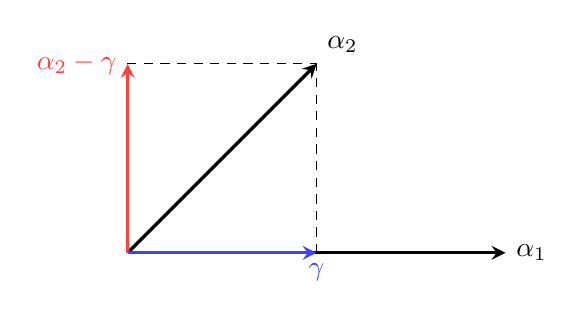
\begin{tikzpicture}[line width=1.2pt,scale=0.8]
			\draw[-stealth] (0,0)--(6,0) node[right] {$ \bm{\alpha}_1 $};
			\draw[-stealth] (0,0)--(3,3) node[above right] {$ \bm{\alpha}_2 $};
			\draw[-stealth,red!75] (0,0)--(0,3) node[left] {$ \bm{\alpha}_2-\bm{\gamma} $};
			\draw[-stealth,blue!75] (0,0)--(3,0) node[below] {$ \bm{\gamma} $};
			\draw[dashed,line width=0] (0,3)--(3,3);
			\draw[dashed,line width=0] (3,0)--(3,3);
			\end{tikzpicture}
	\end{minipage}}
	\qquad
	\subfloat[三维空间正交化]{
		\label{fig-sw}
		\begin{minipage}{8cm}
			\centering
			\tdplotsetmaincoords{60}{110}
			\begin{tikzpicture}[line width=1.2pt,tdplot_main_coords,scale =0.8]
			\draw[->,black!75](0,0,0)--(6,0,0) node[below left] {$\bm{\beta}_1,\bm{\alpha}_1$};
			\draw[->,black!75](0,0,0)--(0,6,0) node[right] {$\bm{\beta}_2$};
			\draw[->,black!75](0,0,0)--(0,0,6) node[right] {$\bm{\beta}_3$};
			\draw[-stealth,red](0,0,0)--(6,0,0);
			\draw[-stealth,red](0,0,0)--(4,6,0) node[below right] {$\bm{\alpha}_2$};
			\draw[-stealth,red](0,0,0)--(2,-2,6) node[below right] {$\bm{\alpha}_3$};
			\draw[-stealth,blue!50](0,0,0)--(0,-2,0) node[left] {$\hat{\bm{\alpha}_3}\prod_{\bm{\beta}_2}{\bm{\alpha}_3}$};
			\draw[-stealth,purple!50](0,0,0)--(2,-2,0);
			\draw[-stealth,orange](0,0,0)--(4,0,0) node[ left] {$\hat{\bm{\alpha}_2}\prod_{\bm{\beta}_1}{\bm{\alpha}_2}$};
			\draw[-stealth,blue!50](0,0,0)--(2,0,0) node[below right] {$\hat{\bm{\alpha}_3}\prod_{\bm{\beta}_1}{\bm{\alpha}_3}$};
			\draw[dashed,line width=0](4,6,0)--(4,0,0);
			\draw[dashed,line width=0](4,6,0)--(0,6,0);
			\draw[dashed,line width=0](2,0,0)--(2,-2,0);
			\draw[dashed,line width=0](2,-2,0)--(0,-2,0);
			\draw[dashed,line width=0](2,-2,6)--(2,-2,0);
			\draw[dashed,line width=0](2,-2,6)--(2,0,0);
			\draw[dashed,line width=0](2,-2,6)--(0,-2,0);
			\draw[dashed,line width=0](2,-2,6)--(0,0,6);
			\end{tikzpicture}
	\end{minipage}}
	\caption{施密特正交化的几何意义}
\end{figure}
\begin{multicols}{2}
\small
\kaishu
\begin{itemize}
	\item 二维平面空间\ 如图\ref{fig-ew}\ 中,\\ 设$ \bm{\alpha}_1,\bm{\alpha}_2 $线性无关,尝试求出$ k $使得:$$ \bm{\alpha}_1\perp\bm{\alpha}_2+k\cdot\bm{\alpha}_1 $$
	\begin{align*}
 \because&\bm{\alpha}_1\perp\bm{\alpha}_2+k\cdot\bm{\alpha}_1 \\ \therefore& (\bm{\alpha}_1,\bm{\alpha}_2+k\bm{\alpha}_1)=0\\
 \therefore& (\bm{\alpha}_1,\bm{\alpha}_2)+(\bm{\alpha}_1,\bm{\alpha}_1)k=0\\
 \therefore& k=-\frac{(\bm{\alpha}_2,\bm{\alpha}_1)}{(\bm{\alpha}_1,\bm{\alpha}_1)}\\
\end{align*}
此时我们令$ \bm{\gamma}=-k\bm{\alpha}_1 $则有$ \bm{\alpha}_1\perp\bm{\alpha}_2-\bm{\gamma} $,已求得与$ \bm{\alpha}_1,\bm{\alpha}_2 $等价的正交基$ \bm{\alpha}_1,\bm{\alpha}_2-\bm{\gamma} $.在二维空间,如图\ref{fig-ew}中$ \bm{\alpha}_2 $在$ \bm{\alpha}_1 $的投影即为$ \bm{\gamma} $.
	\begin{align*}
\mbox{又}\because\bm{\gamma}&=\textstyle{\prod_{\bm{\alpha}_1}{\bm{\alpha}_2}}\displaystyle\cdot\hat{\bm{\alpha}_1}=\frac{(\bm{\alpha}_2,\bm{\alpha}_1)}{|\bm{\alpha}_1|}\cdot\hat{\bm{\alpha}_1}\\&=\frac{(\bm{\alpha}_2,\bm{\alpha}_1)}{|\bm{\alpha}_1|}\cdot\frac{\bm{\alpha}_1}{|\bm{\alpha}_1|}\\
&=\frac{(\bm{\alpha}_2,\bm{\alpha}_1)}{|\bm{\alpha}_1|}\bm{\alpha}_1\\
&=\frac{(\bm{\alpha}_2,\bm{\alpha}_1)}{(\bm{\alpha}_1,\bm{\alpha}_1)}\bm{\alpha}_1
	\end{align*}
则有平面内积空间$ \mathbb{R}^n $中的一组正交基$ \bm{\beta}_,\bm{\beta}_2 $其中
	\begin{align*}
\bm{\beta}_1&=\bm{\alpha}_{1},\\
\bm{\beta}_2&=\bm{\alpha}_2-\bm{\gamma}\\&=\bm{\alpha}_{2}-\dfrac{(\bm{\alpha}_2,\bm{\beta}_1)}{(\bm{\beta}_1,\bm{\beta}_1)}\bm{\beta}_1.	\end{align*}

\item 三维立体空间\ 如图\ref{fig-sw}\ 中,\\设$ \bm{\alpha}_1,\bm{\alpha}_2,\bm{\alpha}_3 $线性无关,以$ \bm{\alpha}_1 $作为正交基中的一个向量$ \bm{\beta}_1 $,并以该向量开始正交化.\\$ \bm{\alpha}_2 $所对应的正交基中的向量$ \bm{\beta}_2 $只需满足$  \bm{\beta}_2\perp \bm{\beta}_1$,按照二维空间的做法进行正交化:(1)作$ \bm{\alpha}_2 $在$ \bm{\alpha}_1 $($ \bm{\beta}_1 $)上的投影$\prod_{\bm{\beta}_1}{\bm{\alpha}_2}$(2)由此可得$ \bm{\beta}_2 =\bm{\alpha}_2-\prod_{\bm{\beta}_1}{\bm{\alpha}_2}\cdot\hat{\bm{\alpha}_2}$.\\$ \bm{\alpha}_3 $所对应的正交基中的向量$ \bm{\beta}_3 $需满足$  \bm{\beta}_3\perp \bm{\beta}_1$且$  \bm{\beta}_3\perp \bm{\beta}_2$因此作$ \bm{\alpha}_3 $在$ \bm{\beta}_1,\bm{\beta}_1 $上的投影$\prod_{\bm{\beta}_1}{\bm{\alpha}_3}$,$\prod_{\bm{\beta}_2}{\bm{\alpha}_3}$.由此可得$ \bm{\beta}_3=\bm{\alpha}_3-\hat{\bm{\alpha}_3}\left(\prod_{\bm{\beta}_1}{\bm{\alpha}_3}+\prod_{\bm{\beta}_2}{\bm{\alpha}_3} \right)  $.综上所述有:\begin{align*}
\bm{\beta}_1&=\bm{\alpha}_{1},\\
\bm{\beta}_2&=\bm{\alpha}_{2}-\dfrac{(\bm{\alpha}_2,\bm{\beta}_1)}{(\bm{\beta}_1,\bm{\beta}_1)}\bm{\beta}_1,\\
\bm{\beta}_3&=\bm{\alpha}_{3}-\dfrac{(\bm{\alpha}_3,\bm{\beta}_1)}{(\bm{\beta}_1,\bm{\beta}_1)}\bm{\beta}_1-\dfrac{(\bm{\alpha}_3,\bm{\beta}_2)}{(\bm{\beta}_2,\bm{\beta}_2)}\bm{\beta}_2-\dfrac{(\bm{\alpha}_3,\bm{\beta}_{2})}{(\bm{\beta}_{2},\bm{\beta}_{2})}\bm{\beta}_{2}.\\
\end{align*}
\end{itemize}
\end{multicols}
\end{theorem}
\begin{method}[标准正交化的方法]
	设$\bm{\alpha}_{1},\bm{\alpha}_{2},\bm{\alpha}_{3},\cdots,\bm{\alpha}_{n} $为内积空间$ \mathbb{R}^n $的一组基,则有以下\textbf{标准正交化}方法:
	\begin{enumerate}
		\item 由格拉姆-施密特正交化定理(定理\ref{gspt})对$\bm{\alpha}_{1},\bm{\alpha}_{2},\bm{\alpha}_{3},\cdots,\bm{\alpha}_{n} $实施正交化得到正交向量组$ \bm{\beta}_{1},\bm{\beta}_{2},\bm{\beta}_{3},\cdots,\bm{\beta}_{n} $;
		\item 由单位化定义(定义\ref{zjhdy})依次对$ \bm{\beta}_{1},\bm{\beta}_{2},\bm{\beta}_{3},\cdots,\bm{\beta}_{n} $单位化,得标准正交基$ \bm{\eta}_1,\bm{\eta}_2,\cdots,\bm{\eta}_n $.
	\end{enumerate}
\end{method}


\subsection{正交矩阵}
\begin{defination}[正交矩阵的定义]
	若$ n $阶\CJKunderdot{实矩阵}$ \bm{A} $满足:\[ \bm{A}^{\mathrm{T}}\bm{A}=\bm{E} ,\]则称$ \bm{A} $为\textbf{正交矩阵}.
	\index{ZJJZ@正交矩阵}
\end{defination}
\begin{feature}[正交矩阵的性质]
	$ n $阶正交矩阵$ \bm{A} $有以下性质:
	\begin{enumerate}
		\item $ \bm{A} $可逆,且$ \bm{A}^{-1}=\bm{A}^{\mathrm{T}} $;
		\item$ \bm{A}^{-1},\bm{A}^{\mathrm{T}} $也是\textbf{正交矩阵};
		\item $ |\bm{A}|=\pm1; $
		\item 正交矩阵的乘积仍为正交矩阵.
	\end{enumerate}
\end{feature}
\begin{theorem}[正交矩阵构造定理]
	设$ \bm{A} $为$ n $阶实矩阵,且$ \bm{A}=[\bm{\alpha}_{1},\bm{\alpha}_{2},\bm{\alpha}_{3},\cdots,\bm{\alpha}_{n}]  $则$  \bm{A} $是正交矩阵的\CJKunderdot{充分必要条件}是列向量$ \bm{\alpha}_{1},\bm{\alpha}_{2},\bm{\alpha}_{3},\cdots,\bm{\alpha}_{n} $构成$ \mathbb{R}^n $的一组标准正交基.
\end{theorem}
\subsection{实对称矩阵的对角化}
\begin{theorem}
	实对称矩阵的特征值必都为常数,且可以取到实的特征向量.
\end{theorem}
\begin{theorem}\label{3.5}
	实对称矩阵$  \bm{A} $属于\CJKunderdot{不同特征值}的特征向量必正交.(由该定理可知若某个特征值只对应一个特征向量时,该特征向量可不进行正交化.)
\end{theorem}
\begin{theorem}\label{SDCJZBKDJH}
	设$  \bm{A} $是一个$ n $阶实对称矩阵,则必定存在\CJKunderdot{正交矩阵}$  \bm{T} $使得\[  \bm{T}^{-1} \bm{A} \bm{T}=\bm{\varLambda} \quad( \bm{\varLambda}\mbox{为对角矩阵}).\]
\end{theorem}
\begin{inference}
	由\ 定理\ref{SDCJZBKDJH}\ 可知:\textbf{实对称矩阵必可对角化}.
\end{inference}
\begin{method}[求正交矩阵的方法]
	\begin{enumerate}
		\item 求出$  \bm{A} $的全部特征值$\lambda_1,\lambda_2,\lambda_3,\cdots,\lambda_n $和属于每一个$ \lambda_i\,(i=1,2,3,\cdots,t) $的特征向量$ \bm{\alpha}_{i1},\bm{\alpha}_{i2},\bm{\alpha}_{i3},\cdots,\bm{\alpha}_{is} $;
		\item 将属于$ \lambda_i\,(i=1,2,3,\cdots,t) $的特征向量$ \bm{\alpha}_{i1},\bm{\alpha}_{i2},\bm{\alpha}_{i3},\cdots,\bm{\alpha}_{is} $正交化和单位化,记为$\bm{\eta}_{i1},\bm{\eta}_{i2},\bm{\eta}_{i3},\cdots,\bm{\eta}_{is} $,他们仍然是属于$ \lambda_i $的线性无关的特征向量;
		\item 由\ 定理\ref{3.5}\ 知,上一步处理后所有特征向量合并之后的向量组仍然为正交的单位向量组,且所含的向量总个数仍为$ n $,以这$ n $个向量为列向量构成的矩阵$  \bm{T} $即为所求.
	\end{enumerate}
\end{method}


\chapter{二次型与二次曲面\\Homogeneous Quadratic Polynomials and Quadrics}
\section{二次型及其标准型}
\subsection{二次型及其矩阵}
\begin{defination}[二次型及二次型矩阵的定义]
	含有$ n $个变量$ x_1,x_2,\cdots,x_n $且系数属于数域$ F $的二次齐次多项式
	\begin{align*}
	f( x_1,x_2,\cdots,x_n )=a_{11}x_1^2+2a_{12}x_1x_2&+\cdots+2a_{1n}x_1x_n\\
	+a_{22}x_2^2&+\cdots+2a_{2n}x_2x_n\\
	&+\cdots\\
	&+a_{nn}x_n^2
	\end{align*}
	称为\textbf{关于数域$ F $的一个$ n $元二次型},简称\textbf{二次型}.
	$ F=\mathbb{R} $时的二次型称为\textbf{实二次型},$ F=\mathbb{C} $时的二次型称为\textbf{复二次型}.
	\index{ECX@二次型} 
	\index{SECX@实二次型} 
	\index{FECX@复二次型} 
	
	下面我们给出二次型的另外一表述方式.令$ a_{ij}=a_{ji}\quad (i<j) $,则$ 2a_{ij}x_ix_j=a_{ij}x_ix_j+a_{ji}x_jx_i $.于是,上述表达式变为
	\begin{align*}
	f( x_1,x_2,\cdots,x_n )=&a_{11}x_1^2+a_{12}x_1x_2+\cdots+a_{1n}x_1x_n+\\
	&a_{21}x_2x_1+a_{22}x_2^2+\cdots+a_{2n}x_2x_n+\cdots\\
	&a_{n1}x_nx_1+a_{n2}x_nx_2+\cdots+a_{nn}x_n^2\\
	=&x_1(a_{11}x_1+a_{12}x_2+\cdots+a_{1n}x_n)+\\
	&x_2(a_{21}x_1+a_{22}x_2+\cdots+a_{2n}x_n)+\cdots\\
	&x_n(a_{n1}x_1+a_{n2}x_2+\cdots+a_{nn}x_n)\\
	=&\begin{bmatrix}
	x_1,x_2,\cdots,x_n
	\end{bmatrix}\begin{bmatrix}
	a_{11}x_1+a_{12}x_2+\cdots+a_{1n}x_n\\
	a_{21}x_1+a_{22}x_2+\cdots+a_{2n}x_n\\
	\vdots\\
	a_{n1}x_1+a_{n2}x_2+\cdots+a_{nn}x_n
	\end{bmatrix}\\
	=&\begin{bmatrix}
	x_1,x_2,\cdots,x_n
	\end{bmatrix}
	\begin{bmatrix}
	a_{11}&a_{12}&\cdots&a_{1n}\\
	a_{21}&a_{22}&\cdots&a_{2n}\\
	\vdots&\vdots& &\vdots\\
	a_{n1}&a_{n2}&\cdots&a_{nn}
	\end{bmatrix}
	\begin{bmatrix}
	x_1\\x_2\\\vdots\\x_n
	\end{bmatrix}
	\end{align*}
其中矩阵\[ \bm{A}=\begin{bmatrix}
a_{11}&a_{12}&\cdots&a_{1n}\\
a_{21}&a_{22}&\cdots&a_{2n}\\
\vdots&\vdots& &\vdots\\
a_{n1}&a_{n2}&\cdots&a_{nn}
\end{bmatrix} \]为对称矩阵.若记\[ \bm{X}=	\begin{bmatrix}
x_1\\x_2\\\vdots\\x_n
\end{bmatrix} \]则二次型可简写成\[ f( x_1,x_2,\cdots,x_n )=\sum_{i=1}^n\sum_{j=1}^na_{ij}x_ix_j=\bm{X}^{\mathbf{T}}\bm{A}\bm{X} \]由于$ a_{ij}=a_{ji} ,$所以\CJKunderdot{矩阵$ \bm{A} $是由二次型唯一确定的对称矩阵},称为\textbf{二次型$ f( x_1,x_2,\cdots,x_n ) $的矩阵}.
\index{ECXFDJZ@二次型$ f( x_1,x_2,\cdots,x_n ) $的矩阵}
\end{defination}
只有平方项的二次型最简单.二次型的\CJKunderdot{基本问题}是研究如何用\textbf{非退化线性替换}把二次型化成只有平方项的问题,简称为\textbf{二次型化平方和的问题}.
\begin{defination}[非退化的线性替换的定义]
	所谓数域$ F $上由变量$x_1,x_2,\cdots,x_n $到变量$ y_1,y_2,\cdots,y_n $的线性替换是指形如\[ 
\begin{bmatrix}
x_1\\x_2\\\vdots\\x_n
\end{bmatrix}
=
\begin{bmatrix}
c_{11}&c_{12}&\cdots&c_{1n}\\
c_{21}&c_{22}&\cdots&c_{2n}\\
\vdots&\vdots& &\vdots\\
c_{n1}&c_{n2}&\cdots&c_{nn}
\end{bmatrix}
\begin{bmatrix}
y_1\\y_2\\\vdots\\y_n
\end{bmatrix}
					\]的一组表达式,其中所有的$ c_{ij} $都在$ F $内.

若系数矩阵\[ \bm{C}=\begin{bmatrix}
c_{11}&c_{12}&\cdots&c_{1n}\\
c_{21}&c_{22}&\cdots&c_{2n}\\
\vdots&\vdots& &\vdots\\
c_{n1}&c_{n2}&\cdots&c_{nn}
\end{bmatrix} \]
\CJKunderdot{可逆},则上述的线性替换称为\textbf{非退化的线性替换}或\textbf{可逆的线性替换}.

同样地,我们记:\[ \bm{X}=\begin{bmatrix}
	x_1\\x_2\\\vdots\\x_n
\end{bmatrix}, \qquad \bm{Y}=\begin{bmatrix}
y_1\\y_2\\\vdots\\y_n
\end{bmatrix}.
 \]则有线性替换\[ \bm{X}=\bm{CY} ,\]与逆向线性替换\[ \bm{Y}=\bm{C}^{-1}\bm{X} .\]
\index{FTHDXXTH@非退化的线性替换}
\index{KNDXXTH@可逆的线性替换}
\end{defination}
二次型化平方和问题的延申:

{\kaishu
设给定的二次型为\[ 	f( x_1,x_2,\cdots,x_n )=\bm{X}^{\mathrm{T}}\bm{AX}. \]
作一个非退化的线性替换\[ \bm{X}=\bm{CY}, \]
就有\[ 	f( x_1,x_2,\cdots,x_n )=(\bm{CY})^{\mathrm{T}}\bm{A}(\bm{CY})=\bm{Y}^{\mathrm{T}}(\bm{C}^{\mathrm{T}}\bm{AC})\bm{Y}=g(y_1,y_2,\cdots,y_n). \]
此时若用$ \bm{B} $表示二次型$ g(y_1,y_2,\cdots,y_n) $的矩阵,由于\[ (\bm{C}^{\mathrm{T}}\bm{AC})^{\mathrm{T}}=\bm{C}^{\mathrm{T}}\bm{A}^{\mathrm{T}}(\bm{C}^{\mathrm{T}})^{\mathrm{T}}=\bm{C}^{\mathrm{T}}\bm{AC} \]则$ \bm{C}^{\mathrm{T}}\bm{AC} $对称,从而有\[ \bm{B}=\bm{C}^{\mathrm{T}}\bm{AC}  \]也为对称矩阵(其中$ \bm{C} $为可逆矩阵).
}
\begin{defination}[矩阵合同的定义]
	设$\bm{A},\bm{B}$为两个$ n\times n $矩阵,若有\CJKunderdot{可逆矩阵} $ \bm{C} $,使得\[ \bm{B}=\bm{C}^{\mathrm{T}}\bm{AC} ,\]则称$ \bm{A} $\textbf{合同于}$ \bm{B} $.
	\index{JZHT@矩阵合同}
	\index{HTJZ@合同矩阵}
\end{defination}
\begin{feature}[合同矩阵的性质]
	矩阵的合同关系满足以下三条性质:
	\begin{enumerate}
		\item 反身性\[ \bm{A}\mbox{合同于}\bm{A}; \]
		\item 对称性\[  \bm{A}\mbox{合同于}\bm{B}\Leftrightarrow\bm{B}\mbox{合同于}\bm{A};\]
		\item 传递性\[ \bm{A}\mbox{合同于}\bm{B} ,\bm{B}\mbox{合同于}\bm{C}\Rightarrow  \bm{A}\mbox{合同于}\bm{C}.\]
	\end{enumerate}
	我们可以发现,矩阵合同与矩阵相似这两种关系都含有\CJKunderdot{矩阵等价}的三条性质,故我们有知道,矩阵合同与矩阵相似是一种特殊的矩阵等价,所以有以下充分条件:
	\begin{itemize}
	\item
$  \mbox{两个矩阵合同}\Rightarrow\mbox{两个矩阵等价}; $
 \item
$  \mbox{两个矩阵相似}\Rightarrow\mbox{两个矩阵等价}. $
\end{itemize}
\end{feature}
\begin{theorem}
	经过非退化的线性替换后,原二次型的矩阵合同于新二次型的矩阵.
\end{theorem}

因此对于矩阵而言,二次型化平方和问题即为求一对角矩阵$ \bm{B} $,使得$ \bm{A},\bm{B} $合同.
\subsection{化二次型为标准型}
\begin{theorem}
	设$ f( x_1,x_2,\cdots,x_n )=\bm{X}^{\mathrm{T}}\bm{AX} $为实二次型,则可作一个非退化的线性替换\[ 
	\left\{
	\begin{array}{c}
	x_1=c_{11}y_1+c_{12}y_2+\cdots+c_{1n}y_n\\
	x_2=c_{21}y_1+c_{22}y_2+\cdots+c_{2n}y_n\\
	\vdots \\
	x_n=c_{n1}y_1+c_{n2}y_2+\cdots+c_{nn}y_n
	\end{array}
	\right.,
 \]其中\[ \bm{C}=\begin{bmatrix}
 c_{11}&c_{12}&\cdots&c_{1n}\\
 c_{21}&c_{22}&\cdots&c_{2n}\\
 \vdots&\vdots& &\vdots\\
 c_{n1}&c_{n2}&\cdots&c_{nn}
 \end{bmatrix} \]为正交矩阵,把$ f( x_1,x_2,\cdots,x_n ) $化成标准型$ \lambda_1 y_1^2+\lambda_2 y_2^2+\cdots+\lambda_n y_n^2 $(平方和),这里$ \lambda_1,\lambda_2,\cdots,\lambda_n $都是$ f( x_1,x_2,\cdots,x_n ) $的矩阵$ \bm{A} $的的特征值.该线性替换(即$ \bm{X}=\bm{TY},\,\bm{T} $为正交矩阵时的线性替换)称为\textbf{正交变换}.\index{ZJBH@正交变换}常利用正交变换的\textbf{保形性}\index{BXX@保形性},解决问题.
\end{theorem}
\begin{theorem}\label{fthxxth}
	数域$ F $上的\CJKunderdot{任意一个二次型}都可以经过非退化线性替换化成平方和的形状(即标准型).即
	\[  f( x_1,x_2,\cdots,x_n )=d_1y_1^2+d_2y_2^2+\cdots+d_ny_n^2 \]等式右端仅有平方项的二次型称为$ f( x_1,x_2,\cdots,x_n ) $的\textbf{标准型}\index{BZX@标准型}.标准型的矩阵为对角矩阵$ \mathrm{diag}(d_1,d_2,\cdots,d_n) $,有
	\[  f( x_1,x_2,\cdots,x_n )=\begin{bmatrix}
	y_1,y_2,\cdots,y_n
	\end{bmatrix}
	\begin{bmatrix}
	d_1&&&\\
	&d_2&&\\
	&&\ddots&\\
	&&&d_n
	\end{bmatrix}\begin{bmatrix}
	y_1\\y_2\\\vdots\\y_n
	\end{bmatrix} .\]
	特别的,若该非退化线性替换为正交变换则有
		\[  f( x_1,x_2,\cdots,x_n )=\begin{bmatrix}
	y_1,y_2,\cdots,y_n
	\end{bmatrix}
	\begin{bmatrix}
	\lambda_1&&&\\
	&\lambda_2&&\\
	&&\ddots&\\
	&&&\lambda_n
	\end{bmatrix}\begin{bmatrix}
	y_1\\y_2\\\vdots\\y_n
	\end{bmatrix} .\]
	其中$ \lambda_1,\lambda_2,\cdots,\lambda_n $都是$ f( x_1,x_2,\cdots,x_n ) $的矩阵$ \bm{A} $的的特征值.
\end{theorem}

定理\,\ref{fthxxth}\,说明任何一个二次型均可通过配方法化成平方和形式.
\begin{inference}
	数域$ F $上的任意对称矩阵都合同于一个对角矩阵.
\end{inference}
\begin{theorem}
	设二次型$f(x_{1},x_{2},\cdots,x_{n})$的矩阵$ \bm{A} $的秩为$ r $,则化成标准型后,对应的矩阵$ \bm{B} $的秩也为$ r $,且说明正好有$ r $个平方项不为零.
	
	所以我们可以称二次型$f(x_{1},x_{2},\cdots,x_{n})$的矩阵$ \bm{A} $的秩为该\textbf{二次型的秩}.
\end{theorem}
\subsection{规范形}

我们知道经过正交变换法与使用配方法的到的标准型不一定相等.这是因为配方法的过程不一定经历过正交化,这会导致图形形状的变化等一系列不便.下面我们将定义一种标准型结果,并且希望该结果由二次型$f(x_{1},x_{2},\cdots,x_{n})$唯一确定.以此我们引出规范形的定义.
\begin{defination}[规范形的定义]

规范形在不同的数域内有不同的表示形式,以下我们将讨论复数域$ \mathbb{C} $与实数域$  \mathbb{R} $内的情况.\index{GFX@规范形}
	\begin{enumerate}
	\item 在$ F=\mathbb{C} $为\textbf{复数域}的情形中进一步讨论.若经过非退化线性替换得到标准型
		\[ f=d_1y_1^2+d_2y_2^2+\cdots+d_ry_r^2\qquad (\mbox{其中}\,d_1,\cdots,d_r\mbox{均不为}\,0).\]考虑到复数均可以开平方则有以下规范化过程:
		\[ 	y_i=\begin{cases}
		\dfrac{1}{\sqrt{d_i}}z_i&i=1,2,\cdots,r \\
		z_i &i=r+1,r+2,\cdots,n
		\end{cases}
		 \]即\[ 
		 \begin{bmatrix}
		 z_1\\\vdots\\z_r\\z_{r+1}\\\vdots\\z_n
		 \end{bmatrix}
		 =
		 \begin{bmatrix}
		 \sqrt{d_1}&&&&&\\
		 &\ddots&&&&\\
		 &&\sqrt{d_r}&&&\\
		 &&&1&&\\
		&&&&\ddots&\\
		 &&&&&1
		 \end{bmatrix}
		 \begin{bmatrix}
		 y_1\\\vdots\\y_r\\y_{r+1}\\\vdots\\y_n
		 \end{bmatrix}
		  \]则它为非退化线性替换,且有规范化后的结果
		 \[ f=z_1^2+z_2^2+\cdots+z_r^2 .\]
		 此处,$ z_1^2+z_2^2+\cdots+z_r^2  $称为\textbf{复二次型$ f $的规范形}.\index{FECXDGFX@复二次型的规范形}
		\item 在$ F=\mathbb{R} $为\textbf{实数域}的情形中进一步讨论.这里我们要求所出现的\CJKunderdot{一切二次型系数都是实数}而且要求所出现的\CJKunderdot{一切二次型系数都是实数}
		
		设$f(x_{1},x_{2},\cdots,x_{n})$的标准型中有$ r $个系数不为零的平方项.根据符号正负重新排列各变量,设
		\[ f=d_1y_1^2+d_2y_2^2+\cdots+d_py_p^2-d_{p+1}y_{p+1}^2-\cdots-d_ry_r^2  (\mbox{其中}\,d_i,i=1,2,\cdots,r,\mbox{均大于}\,0),\]同样地,我们令
		\[ \begin{cases}
	y_i=\dfrac{1}{\sqrt{d_i}}z_i&i=1,2,\cdots,r \\
y_j=z_j &j=r+1,r+2,\cdots,n
\end{cases}
\]则\[ f=z_1^2+\cdots+z_p^2-z_{p+1}^2-\cdots-z_r^2. \]上式右端称为\textbf{实二次型$ f $的规范形}.其中,系数为$ +1 $的平方项有$ p $个,系数为$ -1 $的平方项有$ r-p $个.\index{SECXDGFX@实二次型的规范形}
	\end{enumerate}
\end{defination}
\begin{theorem}[惯性定理]
	任意一个实数域上的二次型$ f( x_1,x_2,\cdots,x_n )=\bm{X}^{\mathrm{T}}\bm{AX} $经过一适当的非退化线性替换可以变成规范型,并且\CJKunderdot{二次型唯一确定规范型}.对于下式\begin{equation*}
f = \underbrace {z_1^2 +  \cdots  + z_p^2}_{\scriptsize \mbox{系数为}+1\mbox{的平方项有}p\mbox{个}}\underbrace { - z_{p + 1}^2 -  \cdots  - z_r^2}_{\scriptsize \mbox{系数为}-1\mbox{的平方项有}r-p\mbox{个}},
\end{equation*}
系数为$ +1 $的平方项个数$ p $称为\textbf{正惯性指数},系数为$ -1 $的平方项个数$ r-p $称为\textbf{负惯性指数}.两者之差称为\textbf{符号差}.\index{ZGXZS@正惯性指数}\index{FGXZS@负惯性指数}\index{FHC@符号差}
\end{theorem}

\section{正定二次型}

本节将继续讨论实二次型.
\begin{defination}[正定二次型的定义]
	给定一个实二次型$f(x_{1},x_{2},\cdots,x_{n})$.
\begin{enumerate}
\item 
	若对任意$n$个\CJKunderdot{不为零的实数}$c_{1},c_{2},\cdots,c_{n}$,总有:
	\begin{itemize}
		\item 	$f(c_{1},c_{2},\cdots,c_{n})>0$,则称$f(x_{1},x_{2},\cdots,x_{n})$为\textbf{正定二次型};\index{ZDECX@正定二次型}
		\item 	$f(c_{1},c_{2},\cdots,c_{n})<0$,则称$f(x_{1},x_{2},\cdots,x_{n})$为\textbf{负定二次型};\index{FDECX@负定二次型}
	\end{itemize}
\item 
	若对任意$n$个\CJKunderdot{实数}$c_{1},c_{2},\cdots,c_{n}$,总有:
	\begin{itemize}
		\item 	$f(c_{1},c_{2},\cdots,c_{n})\geqslant0$,则称$f(x_{1},x_{2},\cdots,x_{n})$为\textbf{半正定二次型};\index{BZDECX@半正定二次型}
		\item 	$f(c_{1},c_{2},\cdots,c_{n})\leqslant0$,则称$f(x_{1},x_{2},\cdots,x_{n})$为\textbf{半负定二次型}.\index{BFDECX@半负定二次型}
	\end{itemize}
\end{enumerate}

因此,正定二次型一定是半正定二次型,半正定二次型不一定是正定二次型,即\[  \mbox{正定二次型} \subsetneqq \mbox{半正定二次型}.\]
显然$f(x_{1},x_{2},\cdots,x_{n})$为负定的当且仅当$-f(x_{1},x_{2},\cdots,x_{n})$为正定的.所以,负定二次型的问题总可以借助正定二次型的理论解决.
\end{defination}
\begin{example}
	二次型$f(x_{1},x_{2},\cdots,x_{n})=x_1^2 + x_2^2 + x_3^2 +  \cdots  + x_{n - 1}^2$是半正定的,但不是正定二次型.实际上,令$ ({x_1},{x_2}, \cdots ,{x_{n - 1}},{x_n}) = (0,0, \cdots ,0,1) \ne 0 $则$ f(x_{1},x_{2},\cdots,x_{n}) $的值为$ 0 $.
\end{example}
\begin{feature}
	非退化线性替换将正定实二次型(负定实二次型)仍变为正定实二次型(负定实二次型).
\end{feature}
\begin{theorem}[正定二次型的判定定理]
	关于正定二次型的判定,有以下\CJKunderdot{等价条件},他们可以互相等价,因此常被用于判定正定二次型.
	
	设有$ n $元实二次型$f(x_{1},x_{2},\cdots,x_{n})=\bm{X}^{\mathrm{T}}\bm{AX}$,则下列命题相互等价:
	\begin{enumerate}
		\item $f(x_{1},x_{2},\cdots,x_{n})$为正定二次型;
		\item $ \bm{A} $的所有特征值都是\CJKunderdot{正实数};
		\item $ \bm{A} $的秩和正惯性指数都是$ n $;
		\item $ \bm{A} $与单位矩阵$ \bm{E} $合同;
		\item 存在可逆矩阵$ \bm{P} $,使得$ \bm{A}=\bm{P}^{\mathrm{T}}\bm{P} $.
	\end{enumerate}
\end{theorem}
\begin{defination}
	如果一个$ n\times n $实对称矩阵$ \bm{A} $所对应的二次型为正定二次型,那么$ \bm{A} $称为\textbf{正定矩阵}.\index{ZDJZ@正定矩阵}
\end{defination}
\begin{feature}
	实正对称矩阵$ \bm{A} $的行列式大于$ 0 $,即$ |\bm{A}|>0 $.
\end{feature}
\begin{defination}[$ \bm{A} $的$ k $阶顺序主子式的定义]
	$ n $阶顺序$ \bm{A}=(a_{ij})_{nn} $的$ k\ (k=1,2,\cdots,n) $阶子式:
	\[{p_k} = \left| {\begin{array}{cccc}
		{{a_{11}}}&{{a_{12}}}& \cdots &{{a_{1k}}}\\
		{{a_{21}}}&{{a_{22}}}& \cdots &{{a_{2k}}}\\
		\vdots & \vdots &{}& \vdots \\
		{{a_{k1}}}&{{a_{k2}}}& \cdots &{{a_{kk}}}
		\end{array}} \right|\]
	称为$ \bm{A} $的$ k $阶\textbf{顺序主子式}.\index{KJSXZZS@$ k $阶顺序主子式}
\end{defination}
\begin{theorem}[实对称矩阵与正定矩阵的关系]
	\,\\
	\begin{itemize}
		\item 实对称矩阵是\CJKunderdot{正定矩阵}$ \Leftrightarrow P_k>0 \ (k=1,2,\cdots,n) $恒成立;
		\item 实对称矩阵是\CJKunderdot{负定矩阵}$ \Leftrightarrow (-1)^kP_k>0 \ (k=1,2,\cdots,n) $恒成立.
	\end{itemize}
\end{theorem}

\section{曲面及其方程}
我们认为:\textbf{曲面}是由\CJKunderdot{一个动点}或一条\CJKunderdot{动曲线}按照一定的条件或规律运动所形成的轨迹.由此可以导出曲面上动点$ P $的坐标$ (x,y,z) $所满足的方程为\index{QM@曲面}
\[
F(x,y,z)=0.
\]

当且仅当$ P $为曲面上的点时其坐标才满足上述方程,那么曲面的几何性质必然可以由该方程反映.因此可以用方程来表述曲面.则把上述方程称为\textbf{曲面的方程}\index{QMDFC@曲面的方程},把上述曲面称为\textbf{方程的图形}\index{FCDTX@方程的图形}.
\subsection{球面及其方程}
\begin{defination}[球面定义]
	空间中到定点的距离等于定长的点的集合称为\textbf{球面}.定点称为\textbf{球心},定长称为\textbf{半径}.
	\index{QM@球面}
	\index{QX@球心}
	\index{BJ@半径}
\end{defination}






%打印索引—————————————
\newpage
\addcontentsline{toc}{chapter}{附录}
\addcontentsline{toc}{section}{索引}
\appendix
\kaishu
\printindex
%———————————————
\end{document}